% nas_compare_v0.0.5 -- v005 draft, assembled 2026-11-17 for a first compilation check (stage C, item 6).
% Same class and preamble as nas_compare_v0.0.3.tex. State of the parts:
%   All parts are v005 drafts (2026-11-17): title (proposal), abstract, introduction, Related Work, problem
%   formulation, P3 and P3Net, Experimental setup, Results (incl. K10), Limitations, Reproducibility, conclusions,
%   appendix (deviations, secondary analyses). No v003 chapter is included any more.
% Main text / supplement split: for now the supplement is an appendix of this file so that every cross-reference
% resolves; it moves to a separate file at stage D. All result tables are in the main text for now.
\documentclass[sigconf,authordraft]{acmart}

\usepackage[T1]{fontenc}
% amsmath/amssymb/amsfonts are already loaded by acmart (newtxmath); loading them again breaks \Bbbk.
\usepackage{graphicx}
\usepackage{textcomp}
\usepackage[table]{xcolor}
\usepackage{longtable}
\usepackage{booktabs}
\usepackage{tabularx}
\usepackage{tikz}
\usetikzlibrary{positioning,arrows.meta}

% Placeholders: anonymous repository link (stage D) and open items in the draft.
\newcommand{\anonrepo}{\textit{[anonymous repository link]}}
\newcommand{\TODO}[1]{\textcolor{red}{[TODO: #1]}}

\acmConference[GECCO '27]{Genetic and Evolutionary Computation Conference}{2027}{TBD}
\acmYear{2027}
\copyrightyear{2027}
\setcopyright{none}
\renewcommand\footnotetextcopyrightpermission[1]{}
\settopmatter{printacmref=false}
\setlength{\headheight}{15.5pt}

\begin{document}

% --- v005 ----------------------------------------------------------------------------------------------------------
% v005 (2026-11-17): title for the "empirical study" narrative (author's decision 2026-11-16). PROPOSAL -- the author
% chooses the final title. Authors and affiliations copied unchanged from chapters/archive/v003/title/main.tex (anonymised at
% stage D).
\title{Linkage Learning for Joint Neural Architecture and Hyperparameter Search: A Pre-registered Study of the
Parameter-less Population Pyramid}

\author{Jędrzej Tomasz Polaczek}
\affiliation{%
    \institution{dept. name of organization (of Aff.)}
    \institution{name of organization (of Aff.)}
    \city{Szczecin}
    \country{Poland}
}
\email{jedrzej.polaczek@gmail.com}

\author{Given Name Surname}
\affiliation{%
    \institution{dept. name of organization (of Aff.)}
    \institution{name of organization (of Aff.)}
    \city{City}
    \country{Country}
}
\email{email address or ORCID}

% v005 (2026-11-17): abstract for the "empirical study" narrative. Every number is from chapters/results/main.tex
% (reports 01-06 in notes/archive/v005/analysis-v005/reports/).
\begin{abstract}
Linkage-learning evolutionary algorithms such as the Parameter-less Population Pyramid (P3) exploit dependencies
between variables, and multi-objective neural architecture search (NAS) is full of them, yet P3 has not been compared
with the methods used for joint architecture and hyperparameter search. We report a pre-registered study of P3 on
this task: P3 alone, P3 with a pairwise surrogate of fitness differences (P3Net) and two variants of it, and P3 with
the eLyMPuS surrogate, against 22 optimisers---NAS-specific, evolutionary, Bayesian, Gaussian-process and
multi-fidelity---on JAHS-Bench-201, NAS-HPO-Bench-II, four FCNet tasks and NAS-Bench-201, at budgets of 50 to 350
evaluations with 30 seeds per cell. P3's standing depends on the budget: at 50 and 100 evaluations it is worse than
most arms on JAHS-Bench-201, random search included, because it spends them on hill-climbing single solutions; at 200
and 350 it is worse than no arm on two of the three JAHS-Bench-201 tasks, and its front is strongest at the accurate
end. The surrogate changes nothing that our tests can detect: P3Net differs from P3 and from its two variants in none of 48
comparisons, and at 1\,000 evaluations, where the surrogate screens nearly 90\,\% of the mixing steps, in none of 12, while raising the
optimiser's time from seconds to about a minute per run. Retraining the selected architectures confirms the benchmark
values to within about one percentage point. Code, run records and the pre-registration are public.
\end{abstract}

\begin{CCSXML}
<ccs2012>
<concept>
<concept_id>10010147.10010178.10010205.10010207</concept_id>
<concept_desc>Computing methodologies~Discrete space search</concept_desc>
<concept_significance>500</concept_significance>
</concept>
<concept>
<concept_id>10010147.10010257.10010293.10010294</concept_id>
<concept_desc>Computing methodologies~Neural networks</concept_desc>
<concept_significance>300</concept_significance>
</concept>
</ccs2012>
\end{CCSXML}

\ccsdesc[500]{Computing methodologies~Discrete space search}
\ccsdesc[300]{Computing methodologies~Neural networks}

\keywords{neural architecture search, hyperparameter optimisation, linkage learning, P3, surrogate,
multi-objective optimisation, benchmarking, pre-registration}

\maketitle

% v005 (2026-11-17): introduction for the "empirical study" narrative. First paragraph kept from v003 (citations
% unchanged); positioning follows chapters/related_work/positioning.tex; numbers from the Results section.
\section{Introduction}
\label{sec:introduction}

Evaluating a candidate network against the true objective -- by training it, through weight sharing, or by
querying a benchmark -- dominates the cost of neural architecture search~\citep{white2023insights,liu2023survey}.
Architecture and training hyperparameters are commonly searched in sequence, yet Zela et al.\ show that they
interact, so the best architecture under one hyperparameter setting need not be the best under
another~\citep{zela2018towards}. Searching both jointly avoids that risk at the price of a larger space, in which
some variables matter only together.

A family of evolutionary algorithms is built around exactly that structure. GOMEA and the Parameter-less Population
Pyramid (P3) learn a linkage tree of dependent variables from the population and keep those groups together during
crossover~\citep{thierens2011optimal,goldman2014parameterless}; on combinatorial benchmarks their advantage over
structure-blind search grows with problem size~\citep{goldman2015fast,qiao2024gomearuntime}. Members of the family
have been applied to architecture search~\citep{denottelander2021localsearch,chebykin2022encas,dahi2026tightening},
and surrogate-assisted variants exist~\citep{dushatskiy2021novelsurrogateassistedevolutionaryalgorithm,przewozniczek2026lympus}.
What is missing is a measurement: how P3 compares, on the joint multi-objective task, with the optimisers that are
actually used for it, at what budget, and at what cost.

\paragraph{This study.} We compare P3 in five forms---canonical P3; P3Net, which replaces the evaluation of mixing steps
by a pairwise surrogate of fitness differences; two variants of P3Net that isolate how the surrogate is used and what
the linkage tree adds to it; and P3 with the eLyMPuS surrogate~\citep{przewozniczek2026lympus}---with 22 optimisers
from NAS, evolutionary computation, Bayesian optimisation and multi-fidelity optimisation. The benchmarks are
JAHS-Bench-201~\citep{bansal2022jahsbench} on three tasks and NAS-HPO-Bench-II~\citep{hirose2021nashpobenchii}, with
four FCNet tasks~\citep{klein2019tabular} that played no part in designing P3Net and NAS-Bench-201 with an energy
objective~\citep{dong2020nasbench201,li2021hwnasbench}. Methods, metrics, tests and seeds were fixed in a
pre-registration before the confirmatory runs, and every sentence about a method's behaviour is tied to a test of the
implementation.

\paragraph{Findings.} P3's standing is set by the budget. With 50 or 100 evaluations it is worse than most arms on
JAHS-Bench-201, random search included, because it spends them on hill-climbing single solutions before any linkage
is used. With 200 or 350 it is worse than no arm on two of the three JAHS-Bench-201 tasks and returns fronts that are
strongest at the accurate end, while population-based methods stay ahead on NAS-HPO-Bench-II. The surrogate changes
nothing that our tests can detect, also at 1\,000 evaluations where it screens most mixing steps, and it raises the
optimiser's own time by an order of magnitude. On the four FCNet tasks P3Net wins more comparisons than it loses.

\paragraph{Contributions.}
\begin{itemize}
    \item A pre-registered comparison of a linkage-learning optimiser with 22 optimisers for joint multi-objective
    NAS and hyperparameter optimisation, on nine search spaces, four budgets and 30 seeds per cell, with
    Holm--Bonferroni-corrected tests, effect sizes, equivalence tests and the optimiser's own time and memory.
    \item A controlled account of what a pairwise surrogate adds to P3: ablations that isolate replacement versus
    gating and the role of the linkage tree, a check that the surrogate-free P3Net is exactly canonical P3, and an
    exploratory budget at which the surrogate acts on most mixing steps.
    \item Evidence on the benchmarks themselves: retraining the selected architectures from scratch, and secondary
    analyses (anytime quality, cost to target, regret, generalisation gaps, sensitivity of the metric).
    \item Code, run records, analysis scripts and the pre-registration, with every table regenerated from the
    records.
\end{itemize}


% --- v005 ----------------------------------------------------------------------------------------------------------
% v005 Related Work, assembled 2026-11-17. Kept verbatim from v003: "Evolutionary NAS with surrogates",
% the pyramid figure and "Joint NAS+HPO benchmarks". New: positioning.tex (replaces v003 "Linkage learning
% and P3", "Surrogate-assisted linkage learning", "Scale dependence", "Closest prior work"),
% compared_methods.tex, llm.tex (replaces the v003 LLM paragraph).

\section{Related Work}
\label{sec:related-work}

\paragraph{Evolutionary NAS with surrogates.} NSGA-Net searches architectures with NSGA-II, training every
candidate fully~\citep{lu2019nsganet}. NSGANetV2 adds an accuracy predictor refined online and inherits weights
from a supernet, cutting the number of fully evaluated architectures to 350~\citep{lu2020nsganetv2}, at the
documented risk of rank disagreement between weight-shared and stand-alone accuracy~\citep{yu2020evaluatingnas}.
White et al.\ identify multi-objective evolutionary search as the most common approach to multi-objective NAS,
with NSGANetV2 as an example~\citep{white2023insights}; Liu et al.\ list learned surrogates as one of several
cost-reduction techniques alongside weight sharing and zero-cost proxies~\citep{liu2023survey}. Later work in
this lineage moves toward ranking-based predictors~\citep{lu2022mosegnas}. None of three recent surveys lists
linkage learning as a distinct NAS method category~\citep{liu2023survey,white2023insights,ozcelik2026survey}.

% v005 stage C draft (2026-11-17): positioning of P3Net in the P3/GOMEA line. Replaces the v003 paragraphs
% "Linkage learning and P3", "Surrogate-assisted linkage learning" and "Closest prior work"
% (chapters/archive/v003/related_work/main.tex); the v003 pyramid figure (fig:p3-pyramid) can be reused unchanged.
% Sources: notes/archive/ga_landscape_2026-07_v003-v005.md §16-§16d; notes/literature.md (literature search 2026-11-16/17). Dahi et al. 2026 is described
% from its supplementary material only (main text not accessible). The sentence on the surrogate result follows the
% current v005 + E1 results and is to be revised if the surrogate study continues.

\paragraph{Linkage learning and P3.} GOMEA and P3 build a linkage tree from statistical dependencies in the
population and use it to guide crossover, so that groups of dependent variables are not
disrupted~\citep{thierens2011optimal,goldman2014parameterless}. P3 replaces a single fixed-size population with a
pyramid of populations (Figure~\ref{fig:p3-pyramid}), adding a level only once existing levels stop improving, so that no population size is
chosen in advance; its evaluation complexity grows more slowly with problem size than that of five
competitors~\citep{goldman2015fast}. Multi-objective variants exist for both: MO-GOMEA~\citep{luong2014mogomea}
and MO-P3, applied to industrial process planning~\citep{przewozniczek2021mop3} and later extended with a Pareto-front
improvement phase~\citep{niemczyk2025pareto}. Unlike the gray-box setting that this line often
exploits~\citep{whitley2016graybox,bouter2023library}, NAS and HPO objectives are not decomposable into cheaply
recomputable subfunctions, so every variation step must be verified by a full evaluation or screened by a surrogate.

\paragraph{Linkage learning in NAS.} Members of this family have been applied to NAS before. den Ottelander et al.\
find MO-GOMEA, NSGA-II, local search and random search indistinguishable on NAS-Bench-101, with MO-GOMEA ahead of
random search on their larger MacroNAS spaces~\citep{denottelander2021localsearch}. ENCAS uses MO-GOMEA to search
cascades of networks drawn from supernetworks~\citep{chebykin2022encas}; Tran et al.\ apply GOMEA to NAS with a
training-free metric in place of training~\citep{tran2023gomeanas}; and Dahi et al., after applying linkage-learning
EAs to architecture search for quantum-circuit transpilation~\citep{dahi2024evolutionary}, use P3 to choose the depth
and layer widths of a small multilayer perceptron within a quantum-optimisation pipeline, a single-objective
architecture search~\citep{dahi2026tightening}. Bartnik adapts the surrogate-assisted P3-GOMEA
of~\citet{dushatskiy2021novelsurrogateassistedevolutionaryalgorithm} to multi-objective NAS on NAS-Bench-201
(accuracy against GPU energy), with an absolute regressor over the genotype as surrogate, an architecture-only
genotype, and MO-LS and surrogate-free MO-P3-GOMEA as baselines~\citep{bartnik2026evolutionary}; we include its two
variants, MO-DSA and MO-PSA, among our comparison arms.

\paragraph{Surrogates and linkage.} CS-GOMEA pairs GOMEA with a convolutional surrogate and names as open the
surrogate's failure to use linkage information in its own construction~\citep{dushatskiy2019csgomea}. LyMPuS builds
the surrogate from the discovered linkage itself and validates it with P3 on NK landscapes, Ising spin glasses and
Max3Sat; its empirical variant, eLyMPuS, discovers the dependency structure incrementally rather than assuming it
known~\citep{przewozniczek2026lympus}. P3Net's surrogate follows eLyMPuS in being relative and
linkage-aware over an incompletely discovered structure, but regresses a continuous fitness difference between
two solutions instead of making a discrete better/worse/ambiguous comparison, which places it closer to CS-GOMEA's
learned model and gives up eLyMPuS's guarantee of recovering the comparison under monotonicity.

\paragraph{Position of this study.} Against this background, P3Net is not the first use of linkage learning, or of
P3, in architecture search. What we have not found is P3 applied to the \emph{joint} multi-objective search over
architecture and training hyperparameters, nor a comparison of a linkage-learning optimiser with the main
Bayesian-optimisation, multi-fidelity and evolutionary methods of multi-objective NAS and HPO under one
pre-registered protocol that also reports the optimiser's own cost. This study supplies that comparison, with P3
in three forms (canonical, with a pairwise surrogate, and with eLyMPuS), on four primary spaces and five further
ones, and it reports where the surrogate does and does not change the outcome. All benchmarks are tabular or
surrogate-based (Section~\ref{sec:setup}).


\begin{figure}[t]
    \centering
    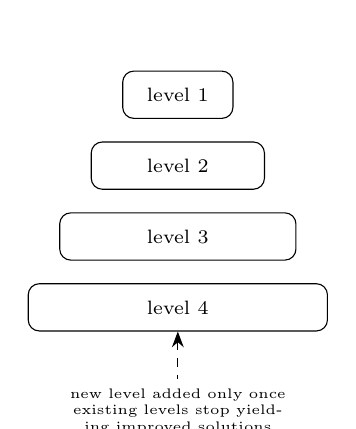
\begin{tikzpicture}[
        lvl/.style={draw, rounded corners, minimum height=6mm, font=\scriptsize, align=center},
    ]
        \node[lvl, minimum width=14mm] (l1) at (0,0)     {level 1};
        \node[lvl, minimum width=22mm] (l2) at (0,-9mm)  {level 2};
        \node[lvl, minimum width=30mm] (l3) at (0,-18mm) {level 3};
        \node[lvl, minimum width=38mm] (l4) at (0,-27mm) {level 4};
        \draw[{Stealth[length=2mm]}-, dashed] (l4.south) -- ++(0,-6mm)
            node[below, font=\tiny, align=center, text width=32mm]
            {new level added only once existing levels stop yielding improved solutions};
    \end{tikzpicture}
    \caption{P3's population pyramid: each level holds a population of growing size; a new level is added only
    when the levels below it stop producing improved solutions.}
    \Description{A vertical stack of four boxes labelled level 1 through level 4, growing wider from top to
    bottom, with an arrow noting that a new level is added only once existing levels stop yielding improved
    solutions.}
    \label{fig:p3-pyramid}
\end{figure}

% v005 stage C draft (2026-11-17): paragraph on the compared methods, to join the v003 Related Work section.
% Citations only for methods actually run in v005 (configs/pipeline/v005.yaml, v005-vizier.yaml). The P3/GOMEA
% positioning paragraphs wait for the author's literature search (notes/archive/v005/plans/v005-todo.md, stage C).

\paragraph{Compared methods.} The comparison covers the main families of multi-objective NAS and HPO optimisers,
each in its published form or the closest available implementation. \emph{NAS-specific search:} NSGA-Net and
NSGANetV2~\citep{lu2019nsganet,lu2020nsganetv2}, REINFORCE~\citep{williams1992reinforce,zoph2017nas} in the
NAS-Bench-201 reference implementation~\citep{dong2020nasbench201} with the MONAS reward~\citep{hsu2018monas} ($\alpha = 0.75$), and regularised evolution~\citep{real2019regularized}.
\emph{Linkage-learning and local search:} canonical P3~\citep{goldman2014parameterless}, P3 with
eLyMPuS~\citep{przewozniczek2026lympus}, the surrogate-assisted P3-GOMEA variants MO-DSA and MO-PSA of
Bartnik~\citep{bartnik2026evolutionary} (after~\citep{dushatskiy2021novelsurrogateassistedevolutionaryalgorithm}), and
multi-objective local search~\citep{denottelander2021localsearch}. \emph{General evolutionary multi-objective
algorithms:} NSGA-III~\citep{deb2014nsga3}, MOEA/D~\citep{zhang2007moead}, and SH-EMOA~\citep{guerreroviu2021bagofbaselines},
which builds on SMS-EMOA~\citep{beume2007smsemoa}. \emph{Bayesian optimisation:} MO-BANANAS~\citep{guerreroviu2021bagofbaselines,white2021bananas},
MOTPE~\citep{ozaki2022motpe} as implemented in Optuna~\citep{akiba2019optuna}, SMAC3 with
ParEGO~\citep{lindauer2022smac3,knowles2006parego}, and three Gaussian-process methods: OSS
Vizier~\citep{song2022ossvizier,song2024vizier}, and qNEHVI and qParEGO in BoTorch~\citep{daulton2021qnehvi,daulton2020qehvi,balandat2020botorch}.
\emph{Multi-fidelity:} Hyperband~\citep{li2018hyperband}, ASHA~\citep{li2020asha} with the multi-objective promotion
rule of MO-ASHA~\citep{schmucker2021moasha}, and the multi-fidelity versions of SH-EMOA, MO-BANANAS (MOSH-BANANAS),
and MO-BOHB~\citep{guerreroviu2021bagofbaselines,falkner2018bohb}. Random search~\citep{bergstra2012random} is the
reference point. Beyond JAHS-Bench-201 and NAS-HPO-Bench-II, the benchmarks are NAS-Bench-201 with energy on an
edge GPU from HW-NAS-Bench as the second objective~\citep{dong2020nasbench201,li2021hwnasbench} and the four FCNet
tabular tasks~\citep{klein2019tabular}. The experimental protocol follows the NAS best-practice
checklist of Lindauer and Hutter~\citep{lindauer2020bestpractices}.


% v005 stage C draft (2026-11-17): the v003 "LLM-based search" paragraph shortened to 4 sentences (v005-plan.md,
% stage C: "Akapit o LLM w Related Work skrócić do 3-4 zdań"). Keys as in v003; the v003 reason "why a
% linkage-learning engine fails to separate from random search" no longer holds and is dropped.

\paragraph{LLM-based search.} Large language models now act as the optimiser~\citep{zheng2023genius,nasir2024llmatic},
as a surrogate~\citep{hao2024llmsurrogate,jawahar2024llmpp}, or as a prior that warm-starts Bayesian
optimisation~\citep{liu2024llambo,zhang2024llmhpo}. Their documented gains concentrate in the early, sparse-data phase
and on small spaces, and several studies trace them to prior knowledge rather than to feedback from
evaluations~\citep{kristiadi2024sober,gupta2025llmbo,ferreira2026centaur}. Linkage learning is the opposite case: it
uses no prior and learns structure only from evaluations. We include no LLM-based arm, because it would draw on
information outside the evaluation budget that binds every other arm, and because NAS-Bench-201 is public and may be
part of the models' training data~\citep{zheng2023genius}.


\paragraph{Joint NAS+HPO benchmarks and their limits.} JAHS-Bench-201 answers queries through a learned surrogate
over a mixed categorical/continuous joint space~\citep{bansal2022jahsbench}; NAS-HPO-Bench-II is a fixed lookup
table over architecture, learning rate, and batch size~\citep{hirose2021nashpobenchii}. Only the latter admits an
exactly enumerable oracle Pareto front, which we exploit for IGD+ (Section~\ref{sec:results}). Guerrero-Viu et
al.\ establish SH-EMOA and MO-BOHB as baselines for this joint setting~\citep{guerreroviu2021bagofbaselines}, none
of them a linkage-learning EA. Both benchmarks share the NAS-Bench-201 cell space~\citep{dong2020nasbench201} and
small-scale image classification. The benchmarking literature documents that search-space design accounts for
much of a method's reported performance and that rankings transfer poorly across
benchmarks~\citep{yang2020nasfrustratinglyhard,mehta2022nasbenchsuite}, that this particular cell space is
redundant and skewed toward already-good architectures~\citep{lopes2023nasbenchdesign}, and that conclusions
transfer inconsistently across task domains~\citep{tu2022nasbench360,duan2021transnasbench101}. Any result on
this family should be read against that.


% v005 (2026-11-17): problem formulation, updated from v003 for the v005 objectives (benchmarks.md BM-1-BM-4,
% decisions #31-#35). Claims: C-13/C-40 (f2 only from evaluation), C-38 (budget), C-39 (duplicates free).
\section{Problem Formulation}
\label{sec:problem-formulation}

\paragraph{Search space.} A genotype $x = (x_1, \dots, x_n) \in \Lambda = \Lambda_1 \times \cdots \times \Lambda_n$
assigns one categorical value to each of $n$ coordinates. In the cell-based spaces the first six coordinates choose
the operation on each edge of the cell; the others choose training hyperparameters. Continuous hyperparameters are
discretised once into a fixed grid, the same for every method, so $\Lambda$ is entirely categorical
(Section~\ref{sec:setup}). Genotypes whose cell has no path from input to output are infeasible; we write
$\Lambda^*$ for the feasible set.

\paragraph{Objectives.} Each $x \in \Lambda^*$ has two objectives to minimise, $\mathbf{f}(x) = (f_1(x), f_2(x))$:
$f_1$ is the validation error after full training and $f_2$ a cost of the model, both read from the benchmark at its
highest fidelity. A method obtains $\mathbf{f}(x)$ only by evaluating $x$; in particular no method is given the cost
$f_2$ of a configuration it has not evaluated. We seek the Pareto front
\[
    \mathcal{P}^* = \bigl\{ x \in \Lambda^* : \nexists\, x' \in \Lambda^*,\;
    \mathbf{f}(x') \preceq \mathbf{f}(x) \wedge \mathbf{f}(x') \neq \mathbf{f}(x) \bigr\},
\]
where $\preceq$ is component-wise $\leq$, and $x'$ \emph{dominates} $x$ when $\mathbf{f}(x') \preceq \mathbf{f}(x)$
and $\mathbf{f}(x') \neq \mathbf{f}(x)$.

\paragraph{Budget.} The cost of a search is the number $b$ of full evaluations. The benchmarks answer
deterministically, so a configuration evaluated again is answered from the run's history
$\mathcal{H}_t = \{(x^{(i)}, \mathbf{f}(x^{(i)}))\}_{i=1}^{t}$ and costs nothing; a run stops at its $b$-th evaluation,
even in the middle of an iteration. The result of a run is $\mathcal{H}_b$, from which its non-dominated set is taken.

% v005 (2026-11-17): P3 and P3Net as implemented in v005 (p3net/v005, cards p3net.md, p3-canonical.md,
% p3net-surrogate.md). Every sentence about behaviour maps to a row of notes/archive/v005/plans/v005-claims.md:
% engine C-01..C-07; canonical C-08, C-11; P3Net C-10, C-12, C-13, C-49, C-51, C-52; variants C-14, C-48 (Z-G1).
% The v003 description (ridge surrogate with cross-validation, kappa, geometric levels with HV-based growth) is
% obsolete and not reused.
\section{P3 and P3Net}
\label{sec:proposed-optimizer}

\paragraph{The P3 engine.} P3 keeps a pyramid of populations without target sizes~\citep{goldman2014parameterless}.
Each iteration adds one new random solution, improves it with a first-improvement hill climber and inserts it into the
lowest level if it is not yet in the pyramid. The solution is then mixed with every level of the pyramid, whether or not
it improved, and it is promoted to the next level only if it dominates its value before mixing and is not yet in the
pyramid. Mixing with a level uses that level's linkage clusters, built with P3's entropy-based distance: all
singletons are used, the root is not, and children of a zero-distance merge are dropped. Clusters are applied smallest
first, ties in random order, each with a donor from the level that differs from the solution on the cluster. With two
objectives, a hill-climbing move and a promotion require Pareto dominance, and a mixing step is kept under the
MO-GOMEA acceptance rule~\citep{luong2014mogomea}: the new solution dominates the current one, has the same
objectives, or is not dominated by the elitist archive of all evaluated solutions. Canonical P3 evaluates every mixing
step that changes the solution and uses no surrogate. P3 has no other parameters.

\paragraph{P3Net.} P3Net keeps this engine and the hill climber on real evaluations, and replaces the evaluations
of mixing steps by a surrogate: mixing with a level runs on predictions, and the solution is evaluated for real once,
after the level. The predicted objectives of a solution reached by a chain of surrogate-accepted steps are, in log
scale, the real objectives of the last really evaluated solution on the chain plus the predicted changes of all steps
since. The surrogate is first
used after the first hill climb has finished; until then mixing uses real evaluations. With the surrogate replaced by
an exact oracle, P3Net reproduces the trajectory of canonical P3, so the surrogate is the only difference between them.

\paragraph{The pairwise surrogate.} The surrogate predicts the difference of both objectives between two solutions,
in log scale, from features of the pair: which variables differ and between which values, and products of such
features for pairs of variables in the same cluster of the current linkage tree, so that the tree decides which
interactions the model can represent. It is antisymmetric by construction. One random forest per objective, with the
library's default hyperparameters and nothing tuned, is trained on all ordered pairs of evaluated solutions, or on
3\,000 of them drawn at random when there are more. Because the cost $f_2$ is predicted like $f_1$, P3Net never sees
the cost of a solution it has not evaluated.

\paragraph{Variants.} Two variants isolate how the surrogate is used and what the linkage tree adds. P3Net-gate uses
the surrogate as a gate instead of a replacement: a mixing step is evaluated for real only when its predicted
objectives would be accepted, and acceptance is then decided on the real values. P3Net-nolink uses the same pairwise
model without the interaction features of the linkage tree.


% --- v005 ----------------------------------------------------------------------------------------------------------
% v005 stage C draft (2026-11-17): Experimental setup. Sources: notes/archive/v005/plans/v005-preregistration.md (§1-§4, §7a),
% notes/archive/v005/plans/v005-sources/benchmarks.md, v005-decisions.md (#25, #30-#37), configs/search_spaces/*_v005.yaml,
% search_spaces/*_genotype.py, configs/pipeline/v005*.yaml (run counts). Methods are cited in Related Work
% (compared_methods.tex); P3Net and its variants are defined in the method section. Hardware: Reproducibility.

\section{Experimental setup}
\label{sec:setup}

\paragraph{Search spaces and objectives.} Table~\ref{tab:v005-spaces} lists the nine search spaces. Every space is a
product of categorical variables, and every method searches the same encoding. The four \emph{primary} spaces carry
the confirmatory tests: JAHS-Bench-201~\citep{bansal2022jahsbench} on its three tasks, CIFAR-10 (C10), Colorectal
Histology (CRC) and Fashion-MNIST (FMN), and NAS-HPO-Bench-II~\citep{hirose2021nashpobenchii} (NHB). On JAHS-Bench-201
the six cell edges are searched together with learning rate (8 log-spaced values in $[10^{-3}, 1]$), weight decay
(6 in $[10^{-5}, 10^{-2}]$), activation and data augmentation; width, depth and resolution are fixed at their
maximum. NHB searches its cell together with learning rate (8 values) and batch size (6). We use NAS-HPO-Bench-II
rather than its successor NAS-HPO-Bench-II-Plus~\citep{hirose2026nashpobenchiiplus}, which answers through learned
surrogates: the tabular original gives the exact Pareto front against which IGD+ is computed. The four FCNet
tasks~\citep{klein2019tabular} form a separate block of spaces that played no part in designing P3Net, and
NAS-Bench-201~\citep{dong2020nasbench201} with edge-GPU energy from HW-NAS-Bench~\citep{li2021hwnasbench} is reported
descriptively. All problems are bi-objective and minimised: $f_1$ is validation error (FCNet: validation MSE) after
full training, and $f_2$ a cost of the model---parameter count on JAHS-Bench-201, computed from the cell because the
benchmark's own model-size output varies with the hyperparameters; training time on NHB and FCNet; inference energy on
NAS-Bench-201. Cells without a path from input to output are rejected for every method.

\begin{table}[t]
    \centering
    \footnotesize
    \setlength{\tabcolsep}{3pt}
    \caption{Search spaces. Variables: number of categorical variables (cell edges + hyperparameters). Front: number
    of points of the exact oracle Pareto front (enumerated once before the runs); JAHS-Bench-201 has none, being a
    surrogate benchmark. Role: P = primary (Q1--Q4 tests), F = FCNet block (Q5 tests), D = descriptive.}
    \label{tab:v005-spaces}
    \begin{tabular}{@{}llrlll@{}}
        \toprule
        \textbf{Space} & \textbf{$f_2$} & \textbf{Var.} & \textbf{Front} & \textbf{Metric} & \textbf{Role} \\
        \midrule
        JAHS-Bench-201 C10, CRC, FMN & parameters & 6\,+\,4 & -- & HV & P \\
        NAS-HPO-Bench-II & training time & 6\,+\,2 & 25 & IGD+ & P \\
        FCNet (Naval, Parkinsons, Protein, Slice) & training time & 0\,+\,9 & 15--28 & IGD+ & F \\
        NAS-Bench-201 & edge-GPU energy & 6\,+\,0 & 30 & IGD+ & D \\
        \bottomrule
    \end{tabular}
\end{table}

\paragraph{Quality metrics.} A run's result is the set of configurations it evaluated at full fidelity, and its
quality is that of the non-dominated subset. Where the oracle front is known we report IGD+~\citep{ishibuchi2015igdplus}
against it, with both objectives normalised to the front's range. On JAHS-Bench-201 we report hypervolume with
objectives normalised by fixed bounds of the space---$f_1$ by $[0, 100]$, $f_2$ by the smallest and largest parameter
count of the task---and reference point $(1.1, 1.1)$, divided by $1.21$ so that it lies in $[0, 1]$. The bounds are
fixed before the runs and no reference depends on the results of any arm.

\paragraph{Arms and tracks.} The \emph{main track} counts the budget in full evaluations and holds P3Net, its three
variants for Q2 (canonical P3 with real evaluations only, P3Net-gate, which uses the surrogate as a gate instead of
a replacement: a mixing step is evaluated for real only when its predicted objectives would be accepted, and
acceptance is then decided on the real values, and P3Net-nolink, whose pair model has no linkage-tree features), P3 with
eLyMPuS, and the 17 comparison arms of Related Work. The three Gaussian-process arms run only at budgets 50 and 100,
for lack of compute. The \emph{multi-fidelity track} (Hyperband, ASHA, and the multi-fidelity SH-EMOA, MOSH-BANANAS and
MO-BOHB) runs on the primary and FCNet spaces with the budget counted as cost in full-evaluation equivalents: training
a configuration to $e$ of $E$ epochs costs $e/E$, and continuing it from $e$ to $e'$ costs $(e'-e)/E$. Lower
fidelities are the benchmarks' values at fewer epochs (on JAHS-Bench-201, surrogate predictions at fewer epochs). In
every arm a configuration proposed again is answered from a cache and costs no budget. Population-based methods use a
population of 20; every baseline runs with its default or published hyperparameters, without tuning.

\paragraph{Budgets and seeds.} Each arm runs at budgets of 50, 100, 200 and 350 with 30 seeds per (space, budget)
cell, in total 26\,400 runs in the main and multi-fidelity tracks and 540 runs of OSS Vizier. The seeds, 62--91, were
never run before the confirmatory runs. An exploratory addendum (E1) runs P3Net, its three Q2 variants and random
search at budget 1000 on the primary spaces with new seeds 92--121; it was planned after the main results were known.

\paragraph{Statistics.} All tests and margins were fixed in the pre-registration. The unit is a (space, budget) cell.
Each comparison of P3Net with another arm is a two-sided Mann--Whitney $U$ test on the 30 per-seed values of the
primary metric---runs with the same seed number are not paired---with Holm--Bonferroni correction over the cell's
comparisons in that question, $\alpha = 0.05$, and Cliff's $\delta$, oriented so that positive favours P3Net. The Q1
family has 17 arms at budgets 50 and 100 and 14 at 200 and 350; Q2 and Q4 have three and five. For the Q2 pairs,
equivalence (Q3) is a two-one-sided test through the 90\,\% percentile bootstrap interval of $\delta$ (4\,000
resamples): \emph{equivalent} if it lies within $(-m, m)$, \emph{different} if it excludes zero, and
\emph{inconclusive} otherwise, with $m = 0.33$ (``small''~\citep{romano2006appropriate}) and, alongside, $m = 0.147$
(``negligible''). Counts of significant comparisons across cells are descriptive; no $p$-values are combined across
cells. No run was excluded.

% v005 stage C draft (2026-11-17), narrative "empirical study" (author's decision 2026-11-16). Numbers from
% notes/analysis-v005/reports/01 (tests), 02 (stage B), 03 (RNG), 04 (E1), all computed from
% results/runs/c674c91e{,-vizier,-e1}/analysis/. Tables: _generated_*.tex (scripts/render_v005_tex.py,
% scripts/analyze_e1_v005.py). Retraining (K10): reports/06, results/retraining/.

\section{Results}
\label{sec:results}

All tests are those of the pre-registration: two-sided Mann--Whitney $U$ per (space, budget) cell, Holm--Bonferroni
within the cell's family, Cliff's $\delta$ oriented so that positive favours P3Net, 30 seeds per arm. Counts of
significant comparisons across cells are descriptive. The four primary spaces are JAHS-Bench-201 on CIFAR-10 (C10),
Colorectal Histology (CRC) and Fashion-MNIST (FMN), measured by normalised hypervolume, and NAS-HPO-Bench-II (NHB),
measured by IGD+ against its exact Pareto front.

\paragraph{Where P3 stands (Q1).} Table~\ref{tab:v005-q1-jahs-c10} and its companions give $\delta$ of P3Net against
the 17 comparison arms. The pattern is set by the budget more than by the space (Figure~\ref{fig:v005-rank-budget}). At $b = 50$ and $100$, P3Net is worse
than 12--17 of the 17 arms on each JAHS space, random search included ($\delta$ between $-0.43$ and $-0.68$), and
better than none; on NHB nearly all comparisons are not significant. At $b = 200$ and $350$ the picture reverses on
CRC and FMN: P3Net is worse than no arm and better than 2--8 of the 14, and its median ranks first or second of 19
arms in three of these four cells. C10 stays harder: at $b = 350$ P3Net is better than one arm and worse than four.
On NHB at $b = 350$ it is better than three and worse than five, with population-based evolutionary methods
(NSGANetV2, NSGA-III, SH-EMOA) ahead. Over all 16 cells, the arms most often better than P3Net are MO-BANANAS,
NSGA-Net, NSGA-III and SH-EMOA (9 cells each) and NSGANetV2 (8). The front P3Net returns is strong at its accurate end
and weaker at its cheap end: in the hypervolume decomposition on JAHS at $b = 350$ it ranks 7th, 3rd and 3rd of 24
arms on the accurate end of C10, CRC and FMN, against 15th, 11th and 4th on the cheap end
(Figure~\ref{fig:v005-fronts} shows the fronts of median runs in one such cell). The Gaussian-process
arms, run only up to $b = 100$, are among the strongest arms at those budgets: OSS Vizier has the best median of the 22 arms in 11 of
the 18 (space, budget) cells of all nine spaces (Table~\ref{tab:v005-s-gp}).

\paragraph{What the surrogate contributes (Q2, Q3).} No comparison of P3Net with canonical P3, P3Net-gate or
P3Net-nolink is significant (0 of 48; Table~\ref{tab:v005-q2-q3}), and P3Net is equivalent to its two variants at
the margin $m = 0.33$ in all 16 cells. This equivalence is largely mechanical. P3Net spends its budget on the
first-improvement hill climber and reaches the mixing stage late: the median number of mixing steps per run on the
primary spaces is 0, 0, 1 and 8 at $b = 50$, 100, 200 and 350, so P3Net-gate and P3Net-nolink end with the same final
value as P3Net in 94.6\,\% and 96.0\,\% of runs. With no mixing step P3Net \emph{is} canonical P3: the surrogate
takes one draw from the random generator when it is built, which shifts the random stream, and with that offset
removed the two produce identical histories (6 of 6 runs checked; without it, canonical P3 diverges in 5 of
the 6). That P3Net and canonical P3 end identically in only
5.8\,\% of runs therefore reflects mostly their different random streams, not surrogate decisions, and at these
budgets the Q1 results describe canonical P3 as much as P3Net.

\paragraph{The surrogate with room to act (E1, exploratory).} To see whether the surrogate matters once it acts, an
exploratory addendum ran the four P3 variants and random search at $b = 1000$ on new seeds
(Table~\ref{tab:v005-e1}). There P3Net takes 91--228 mixing steps per run, of which the surrogate screens 86--92\,\%,
and runs are no longer copies of each other (3--17\,\% identical to canonical P3). Still, none of the 12
comparisons is significant; at $m = 0.33$ nine are equivalent, two inconclusive, and one---canonical P3 on C10,
$\delta = -0.26$---has a confidence interval excluding zero in canonical P3's favour, while its Mann--Whitney test is
not significant ($p = 0.084$). The surrogate raises P3Net's optimiser time from 0--2.5\,s to 50--85\,s per run. All
four variants beat random search ($\delta$ 0.92--1.00). Within the design tested, a pairwise regressor of fitness
differences, the surrogate does not improve P3 on these benchmarks.

\paragraph{Multi-fidelity methods (Q4).} With the budget counted in full-evaluation equivalents, P3Net is worse than
all five multi-fidelity arms at $b = 50$ and $100$ on the three JAHS spaces (Table~\ref{tab:v005-q4-mf}). At
$b = 350$ it is better than ASHA, Hyperband and MOSH-BANANAS on CRC and FMN, and on FMN also than SH-EMOA. On NHB most
comparisons are not significant. Overall P3Net is better in 12, worse in 33 and indistinguishable in 35 of 80
comparisons.

\paragraph{Spaces outside the design loop (Q5).} On the four FCNet tasks, which played no part in designing P3Net,
the balance is more favourable than on the primary spaces: P3Net is better in 64, worse in 36 and indistinguishable in
148 of 248 comparisons (Table~\ref{tab:v005-q5-fcnet}). Protein structure is the exception, with 8 better against 21
worse. The primary-space result therefore does not transfer as a single verdict; it holds per space and per budget.

\paragraph{Optimiser cost (Q6).} Table~\ref{tab:v005-q6-costs} separates the optimiser's own time from the
benchmark queries. The arms strongest at small budgets are also the most expensive
(Figure~\ref{fig:v005-quality-cost}): at $b = 100$ on C10, OSS Vizier
needs a median of 1\,160\,s per run and 14\,GB of memory (up to 25\,GB elsewhere), NSGANetV2 624\,s, and qNEHVI 160\,s, against 0.3\,s for
P3Net; at $b = 350$ NSGANetV2 needs 2\,825\,s against 5.7\,s. On a tabular benchmark this cost dominates the run; in
real NAS, where one evaluation is a training run, it does not---the ratio matters when evaluations are cheap.
Measured in evaluations instead (Table~\ref{tab:v005-s-ctt}), P3Net is slow to reach a high target at $b = 350$: on
JAHS it reaches 99\,\% of the best median final HV in 67, 87 and 90\,\% of runs on C10, CRC and FMN, after a
median of 124, 135 and 127 evaluations, whereas most comparison arms reach it in all or nearly all runs and sooner
(on FMN after about 20). On NHB the target is hard for every arm: 95\,\% of the best median IGD+ is reached by at
most half of the runs of any arm (NSGANetV2) and by 3\,\% of P3Net's.

\paragraph{NAS-Bench-201 (descriptive).} With energy as the second objective, NAS-Bench-201 separates methods: median
IGD+ at $b = 350$ ranges from 0.0096 (NSGANetV2) to 0.0375 (MO-DSA), and the order of arms is stable between
$b = 200$ and 350 (Spearman 0.95). P3Net ranks 12th of 19 at both budgets, between canonical P3 and random search
(Table~\ref{tab:v005-s-nb201}).

\paragraph{P3 with eLyMPuS (Q7, supplement).} P3 with the eLyMPuS surrogate is worse than canonical P3 in 33 of 36
cells ($\delta$ down to $-0.38$; Table~\ref{tab:v005-s-q7}): at these budgets, discovering dependencies costs evaluations that canonical P3 spends
on search.

\paragraph{Secondary analyses (supplement).} The pre-registered descriptive analyses agree with the tests.
The anytime curves (Figure~\ref{fig:v005-s-anytime}) show why P3 trails at small budgets: on JAHS, P3Net and canonical
P3 rise late and in steps, the first evaluations going into hill-climbing single solutions, and they join the leading
group only after about 110--160 evaluations on CRC and FMN, and on C10 end below the best arm. Simple regret of $f_1$ at $b = 350$
(Table~\ref{tab:v005-s-regret}) matches the strong accurate end: on CRC and FMN P3Net's median regret (0.29 and
0.15 percentage points) is within 0.01 of the lowest of any arm, while on C10 and NHB it lies inside the range of the
other arms. The gap between test and validation error of the final fronts (Table~\ref{tab:v005-s-gap}) varies far more
between spaces than between arms (CRC $+1.0$ to $+1.9$, NAS-Bench-201 $-2.4$ to $-2.9$ percentage points). Recomputing HV with the reference points
$(1.05, 1.05)$ and $(1.2, 1.2)$ leaves the order of arms practically unchanged (Spearman $\ge 0.992$ in all 12 JAHS
cells) and P3Net's rank unchanged (Table~\ref{tab:v005-s-hvsens}). Every arm exhausts its budget in every run except
REINFORCE (15.8\,\% of runs; its policy converges and re-proposes one configuration), MO-DSA and MO-PSA (80.9 and
88.0\,\%; 1\,000 iterations without a new evaluation), MOTPE (99.6\,\%) and SH-EMOA (MF), whose schedule ends just
short of the budget (Table~\ref{tab:v005-s-budget}).

\paragraph{Retraining the knee points.} To check that the tabular values carry over to real training, we retrained
from scratch, once each, the knee point of every arm's median run at its largest budget on NAS-Bench-201 and
NAS-HPO-Bench-II with the benchmarks' training protocols (40 trainings for 49 knee points, as arms with the same
knee share one). On NAS-Bench-201 the retrained validation accuracy is close to the benchmark's value: mean
difference $-0.10$ percentage points, median absolute difference 0.24, at most 0.56, and Spearman 0.75 between the
two over the 16 trainings. On NAS-HPO-Bench-II it is lower by 0.88 points on average (median absolute difference 0.96,
at most 3.4), with Spearman 0.92 over 24 trainings; our network for this benchmark is built with a different code
base from the authors' (pre-registration \S8). Many knees lie close together (16 of 22 within 0.6 points on
NAS-Bench-201; 13 of 27 within one point of P3Net's on NAS-HPO-Bench-II), so a single training per knee reorders them: P3Net's knee ranks 9th among the arms by the benchmark's value on both benchmarks and
15th of 22 and 16th of 27 after retraining. The retraining thus confirms the benchmark values to within about a
point, and does not separate the arms.

% GENERATED by implementation/experiments/scripts/render_v005_figures.py.
% Do not edit by hand -- regenerate from results/runs/<root>/ instead.

\begin{figure*}[t]
    \centering
    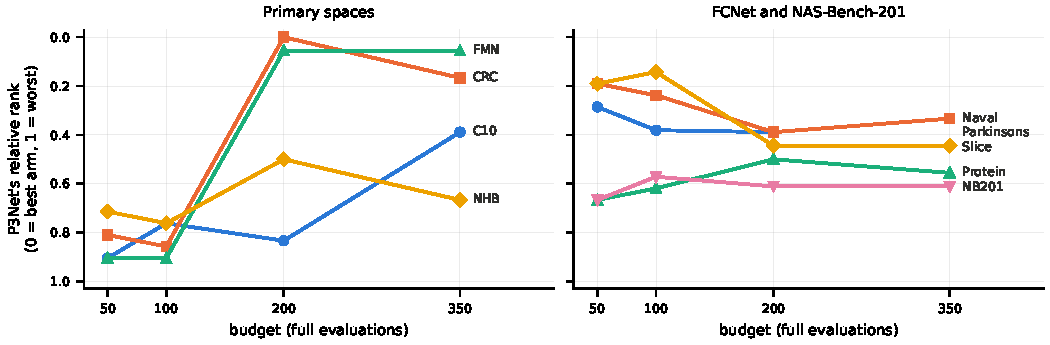
\includegraphics[width=\textwidth]{figures/rank__p3net__by_budget.pdf}
    \caption{P3Net's standing by budget: relative rank of its median final quality among the main-track arms run in the cell (0 = best, 1 = worst; 22 arms at $b \le 100$, 19 at $b \ge 200$, ties share the lower rank). Left: the primary spaces; right: the FCNet tasks and NAS-Bench-201.}
    \Description{Two line charts of P3Net's relative rank against the budget, one line per search space: on most spaces the rank improves from near the worst at 50 evaluations to near the best at 200 or 350.}
    \label{fig:v005-rank-budget}
\end{figure*}

\begin{figure*}[t]
    \centering
    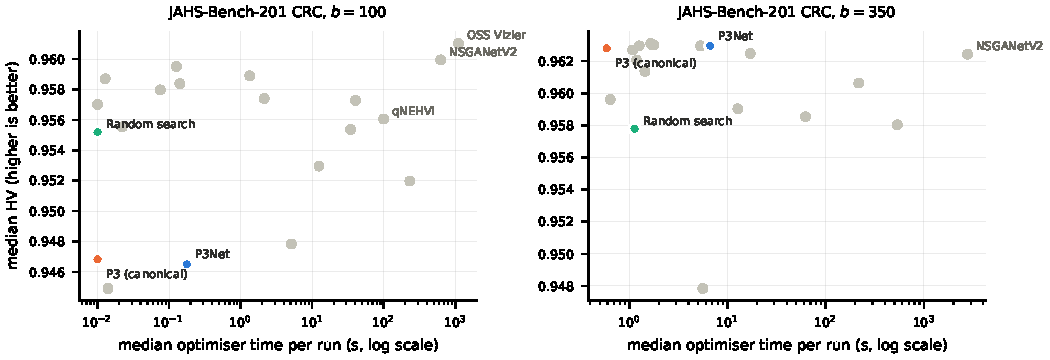
\includegraphics[width=\textwidth]{figures/quality_vs_cost__colorectal.pdf}
    \caption{Quality against the optimiser's own cost on JAHS-Bench-201 Colorectal Histology: median HV over 30 seeds and median optimiser wall-clock time per run without benchmark queries (log scale), one point per main-track arm, at $b = 100$ (with the Gaussian-process arms) and $b = 350$; times below 0.01\,s are drawn at 0.01\,s. Coloured: P3Net, canonical P3 and random search; grey: the other arms.}
    \Description{Two scatter plots of median hypervolume against optimiser time on a log axis; the Gaussian-process arms and NSGANetV2 are the most expensive, P3Net and canonical P3 among the cheapest.}
    \label{fig:v005-quality-cost}
\end{figure*}

\begin{figure}[t]
    \centering
    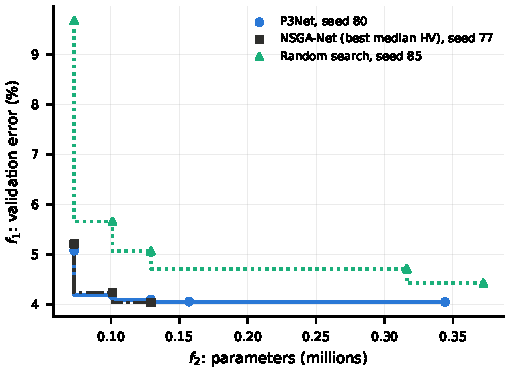
\includegraphics[width=\linewidth]{figures/fronts__colorectal__budget350.pdf}
    \caption{Final non-dominated fronts of the median run (by HV) of P3Net, of the arm with the best median HV (NSGA-Net) and of random search, JAHS-Bench-201 Colorectal Histology, $b = 350$; both objectives are minimised.}
    \Description{Step plots of validation error against parameter count for three fronts; the fronts of P3Net and of the best arm both reach about four percent error, random search's front stays higher.}
    \label{fig:v005-fronts}
\end{figure}

% GENERATED by implementation/experiments/scripts/render_v005_tex.py.
% Do not edit by hand -- regenerate from results/runs/<root>/analysis/ instead.

\begin{table}[t]
    \centering
    \footnotesize
    \setlength{\tabcolsep}{2pt}
    \caption{Q1, JAHS-Bench-201 CIFAR-10: Cliff's $\delta$ of P3Net vs.\ each arm, 30 seeds each; positive (blue) favours P3Net, negative (red) the arm; darker is larger $|\delta|$. Boxed: rejects $H_0$ after Holm--Bonferroni within the (space, budget) cell, two-sided Mann--Whitney $U$, $\alpha=0.05$. Metric: normalised hypervolume (higher is better). Holm family: 17 arms at budgets 50 and 100, 14 at 200 and 350 (OSS Vizier, qNEHVI and qParEGO run only at 50 and 100; -- = not run).}
    \label{tab:v005-q1-jahs-c10}
    \begin{tabular}{@{}lcccc@{}}
        \toprule
        \textbf{Arm} & \textbf{50} & \textbf{100} & \textbf{200} & \textbf{350} \\
        \midrule
        MO-DSA & \colorbox[HTML]{FBDCDB}{\makebox[2.2em]{\textcolor{black}{-0.28}}} & \colorbox[HTML]{FDEEED}{\makebox[2.2em]{\textcolor{black}{-0.00}}} & \colorbox[HTML]{FBDCDB}{\makebox[2.2em]{\textcolor{black}{-0.13}}} & \colorbox[HTML]{86B6EF}{\makebox[2.2em]{\textcolor{black}{+0.35}}} \\
        MO-PSA & \colorbox[HTML]{FBDCDB}{\makebox[2.2em]{\textcolor{black}{-0.24}}} & \colorbox[HTML]{FBDCDB}{\makebox[2.2em]{\textcolor{black}{-0.15}}} & \colorbox[HTML]{FBDCDB}{\makebox[2.2em]{\textcolor{black}{-0.18}}} & \colorbox[HTML]{86B6EF}{\makebox[2.2em]{\textcolor{black}{+0.32}}} \\
        \midrule
        NSGA-Net & \fcolorbox[HTML]{000000}{F2A3A2}{\makebox[2.2em]{\textcolor{black}{\textbf{-0.45}}}} & \fcolorbox[HTML]{000000}{E34948}{\makebox[2.2em]{\textcolor{white}{\textbf{-0.51}}}} & \fcolorbox[HTML]{000000}{E34948}{\makebox[2.2em]{\textcolor{white}{\textbf{-0.60}}}} & \fcolorbox[HTML]{000000}{E34948}{\makebox[2.2em]{\textcolor{white}{\textbf{-0.64}}}} \\
        NSGANetV2 & \fcolorbox[HTML]{000000}{E34948}{\makebox[2.2em]{\textcolor{white}{\textbf{-0.65}}}} & \fcolorbox[HTML]{000000}{941F1F}{\makebox[2.2em]{\textcolor{white}{\textbf{-0.77}}}} & \fcolorbox[HTML]{000000}{E34948}{\makebox[2.2em]{\textcolor{white}{\textbf{-0.68}}}} & \colorbox[HTML]{F2A3A2}{\makebox[2.2em]{\textcolor{black}{-0.40}}} \\
        REINFORCE & \colorbox[HTML]{F2A3A2}{\makebox[2.2em]{\textcolor{black}{-0.31}}} & \colorbox[HTML]{FBDCDB}{\makebox[2.2em]{\textcolor{black}{-0.16}}} & \colorbox[HTML]{CDE2FB}{\makebox[2.2em]{\textcolor{black}{+0.28}}} & \fcolorbox[HTML]{000000}{3987E5}{\makebox[2.2em]{\textcolor{white}{\textbf{+0.69}}}} \\
        RegEvo & \fcolorbox[HTML]{000000}{E34948}{\makebox[2.2em]{\textcolor{white}{\textbf{-0.50}}}} & \fcolorbox[HTML]{000000}{E34948}{\makebox[2.2em]{\textcolor{white}{\textbf{-0.54}}}} & \fcolorbox[HTML]{000000}{F2A3A2}{\makebox[2.2em]{\textcolor{black}{\textbf{-0.43}}}} & \colorbox[HTML]{FBDCDB}{\makebox[2.2em]{\textcolor{black}{-0.18}}} \\
        \midrule
        MO-LS & \fcolorbox[HTML]{000000}{F2A3A2}{\makebox[2.2em]{\textcolor{black}{\textbf{-0.48}}}} & \fcolorbox[HTML]{000000}{E34948}{\makebox[2.2em]{\textcolor{white}{\textbf{-0.63}}}} & \colorbox[HTML]{F2A3A2}{\makebox[2.2em]{\textcolor{black}{-0.40}}} & \colorbox[HTML]{EAF2FC}{\makebox[2.2em]{\textcolor{black}{+0.02}}} \\
        SH-EMOA & \fcolorbox[HTML]{000000}{941F1F}{\makebox[2.2em]{\textcolor{white}{\textbf{-0.79}}}} & \fcolorbox[HTML]{000000}{E34948}{\makebox[2.2em]{\textcolor{white}{\textbf{-0.65}}}} & \fcolorbox[HTML]{000000}{E34948}{\makebox[2.2em]{\textcolor{white}{\textbf{-0.67}}}} & \fcolorbox[HTML]{000000}{E34948}{\makebox[2.2em]{\textcolor{white}{\textbf{-0.61}}}} \\
        NSGA-III & \fcolorbox[HTML]{000000}{E34948}{\makebox[2.2em]{\textcolor{white}{\textbf{-0.62}}}} & \fcolorbox[HTML]{000000}{E34948}{\makebox[2.2em]{\textcolor{white}{\textbf{-0.62}}}} & \fcolorbox[HTML]{000000}{E34948}{\makebox[2.2em]{\textcolor{white}{\textbf{-0.57}}}} & \fcolorbox[HTML]{000000}{E34948}{\makebox[2.2em]{\textcolor{white}{\textbf{-0.53}}}} \\
        MOEA/D & \fcolorbox[HTML]{000000}{E34948}{\makebox[2.2em]{\textcolor{white}{\textbf{-0.56}}}} & \fcolorbox[HTML]{000000}{F2A3A2}{\makebox[2.2em]{\textcolor{black}{\textbf{-0.43}}}} & \colorbox[HTML]{FBDCDB}{\makebox[2.2em]{\textcolor{black}{-0.22}}} & \colorbox[HTML]{CDE2FB}{\makebox[2.2em]{\textcolor{black}{+0.26}}} \\
        \midrule
        MO-BANANAS & \fcolorbox[HTML]{000000}{941F1F}{\makebox[2.2em]{\textcolor{white}{\textbf{-0.71}}}} & \fcolorbox[HTML]{000000}{E34948}{\makebox[2.2em]{\textcolor{white}{\textbf{-0.69}}}} & \fcolorbox[HTML]{000000}{E34948}{\makebox[2.2em]{\textcolor{white}{\textbf{-0.56}}}} & \fcolorbox[HTML]{000000}{F2A3A2}{\makebox[2.2em]{\textcolor{black}{\textbf{-0.48}}}} \\
        MOTPE & \fcolorbox[HTML]{000000}{E34948}{\makebox[2.2em]{\textcolor{white}{\textbf{-0.68}}}} & \fcolorbox[HTML]{000000}{E34948}{\makebox[2.2em]{\textcolor{white}{\textbf{-0.64}}}} & \fcolorbox[HTML]{000000}{F2A3A2}{\makebox[2.2em]{\textcolor{black}{\textbf{-0.47}}}} & \colorbox[HTML]{FDEEED}{\makebox[2.2em]{\textcolor{black}{-0.07}}} \\
        SMAC3-ParEGO & \fcolorbox[HTML]{000000}{E34948}{\makebox[2.2em]{\textcolor{white}{\textbf{-0.59}}}} & \fcolorbox[HTML]{000000}{E34948}{\makebox[2.2em]{\textcolor{white}{\textbf{-0.56}}}} & \colorbox[HTML]{F2A3A2}{\makebox[2.2em]{\textcolor{black}{-0.40}}} & \colorbox[HTML]{FDEEED}{\makebox[2.2em]{\textcolor{black}{-0.01}}} \\
        OSS Vizier & \fcolorbox[HTML]{000000}{F2A3A2}{\makebox[2.2em]{\textcolor{black}{\textbf{-0.42}}}} & \fcolorbox[HTML]{000000}{E34948}{\makebox[2.2em]{\textcolor{white}{\textbf{-0.55}}}} & -- & -- \\
        qNEHVI & \fcolorbox[HTML]{000000}{E34948}{\makebox[2.2em]{\textcolor{white}{\textbf{-0.66}}}} & \fcolorbox[HTML]{000000}{F2A3A2}{\makebox[2.2em]{\textcolor{black}{\textbf{-0.44}}}} & -- & -- \\
        qParEGO & \fcolorbox[HTML]{000000}{E34948}{\makebox[2.2em]{\textcolor{white}{\textbf{-0.50}}}} & \fcolorbox[HTML]{000000}{E34948}{\makebox[2.2em]{\textcolor{white}{\textbf{-0.52}}}} & -- & -- \\
        \midrule
        Random search & \fcolorbox[HTML]{000000}{E34948}{\makebox[2.2em]{\textcolor{white}{\textbf{-0.68}}}} & \fcolorbox[HTML]{000000}{E34948}{\makebox[2.2em]{\textcolor{white}{\textbf{-0.53}}}} & \colorbox[HTML]{FBDCDB}{\makebox[2.2em]{\textcolor{black}{-0.22}}} & \colorbox[HTML]{CDE2FB}{\makebox[2.2em]{\textcolor{black}{+0.29}}} \\
        \bottomrule
    \end{tabular}
\end{table}

\begin{table}[t]
    \centering
    \footnotesize
    \setlength{\tabcolsep}{2pt}
    \caption{Q1, JAHS-Bench-201 Colorectal Histology: Cliff's $\delta$ of P3Net vs.\ each arm, 30 seeds each; positive (blue) favours P3Net, negative (red) the arm; darker is larger $|\delta|$. Boxed: rejects $H_0$ after Holm--Bonferroni within the (space, budget) cell, two-sided Mann--Whitney $U$, $\alpha=0.05$. Metric: normalised hypervolume (higher is better). Holm family: 17 arms at budgets 50 and 100, 14 at 200 and 350 (OSS Vizier, qNEHVI and qParEGO run only at 50 and 100; -- = not run).}
    \label{tab:v005-q1-jahs-crc}
    \begin{tabular}{@{}lcccc@{}}
        \toprule
        \textbf{Arm} & \textbf{50} & \textbf{100} & \textbf{200} & \textbf{350} \\
        \midrule
        MO-DSA & \colorbox[HTML]{FBDCDB}{\makebox[2.2em]{\textcolor{black}{-0.23}}} & \colorbox[HTML]{FBDCDB}{\makebox[2.2em]{\textcolor{black}{-0.12}}} & \fcolorbox[HTML]{000000}{3987E5}{\makebox[2.2em]{\textcolor{white}{\textbf{+0.53}}}} & \fcolorbox[HTML]{000000}{3987E5}{\makebox[2.2em]{\textcolor{white}{\textbf{+0.68}}}} \\
        MO-PSA & \colorbox[HTML]{FBDCDB}{\makebox[2.2em]{\textcolor{black}{-0.22}}} & \colorbox[HTML]{FBDCDB}{\makebox[2.2em]{\textcolor{black}{-0.14}}} & \fcolorbox[HTML]{000000}{3987E5}{\makebox[2.2em]{\textcolor{white}{\textbf{+0.59}}}} & \fcolorbox[HTML]{000000}{3987E5}{\makebox[2.2em]{\textcolor{white}{\textbf{+0.67}}}} \\
        \midrule
        NSGA-Net & \fcolorbox[HTML]{000000}{E34948}{\makebox[2.2em]{\textcolor{white}{\textbf{-0.52}}}} & \fcolorbox[HTML]{000000}{F2A3A2}{\makebox[2.2em]{\textcolor{black}{\textbf{-0.42}}}} & \colorbox[HTML]{CDE2FB}{\makebox[2.2em]{\textcolor{black}{+0.21}}} & \colorbox[HTML]{FDEEED}{\makebox[2.2em]{\textcolor{black}{-0.07}}} \\
        NSGANetV2 & \fcolorbox[HTML]{000000}{E34948}{\makebox[2.2em]{\textcolor{white}{\textbf{-0.67}}}} & \fcolorbox[HTML]{000000}{E34948}{\makebox[2.2em]{\textcolor{white}{\textbf{-0.53}}}} & \colorbox[HTML]{CDE2FB}{\makebox[2.2em]{\textcolor{black}{+0.16}}} & \colorbox[HTML]{CDE2FB}{\makebox[2.2em]{\textcolor{black}{+0.27}}} \\
        REINFORCE & \colorbox[HTML]{FBDCDB}{\makebox[2.2em]{\textcolor{black}{-0.25}}} & \colorbox[HTML]{FBDCDB}{\makebox[2.2em]{\textcolor{black}{-0.12}}} & \fcolorbox[HTML]{000000}{184F95}{\makebox[2.2em]{\textcolor{white}{\textbf{+0.70}}}} & \fcolorbox[HTML]{000000}{184F95}{\makebox[2.2em]{\textcolor{white}{\textbf{+0.86}}}} \\
        RegEvo & \fcolorbox[HTML]{000000}{F2A3A2}{\makebox[2.2em]{\textcolor{black}{\textbf{-0.44}}}} & \colorbox[HTML]{F2A3A2}{\makebox[2.2em]{\textcolor{black}{-0.36}}} & \fcolorbox[HTML]{000000}{86B6EF}{\makebox[2.2em]{\textcolor{black}{\textbf{+0.42}}}} & \colorbox[HTML]{86B6EF}{\makebox[2.2em]{\textcolor{black}{+0.36}}} \\
        \midrule
        MO-LS & \colorbox[HTML]{FBDCDB}{\makebox[2.2em]{\textcolor{black}{-0.28}}} & \colorbox[HTML]{F2A3A2}{\makebox[2.2em]{\textcolor{black}{-0.36}}} & \colorbox[HTML]{CDE2FB}{\makebox[2.2em]{\textcolor{black}{+0.22}}} & \colorbox[HTML]{86B6EF}{\makebox[2.2em]{\textcolor{black}{+0.36}}} \\
        SH-EMOA & \fcolorbox[HTML]{000000}{E34948}{\makebox[2.2em]{\textcolor{white}{\textbf{-0.63}}}} & \fcolorbox[HTML]{000000}{F2A3A2}{\makebox[2.2em]{\textcolor{black}{\textbf{-0.46}}}} & \colorbox[HTML]{CDE2FB}{\makebox[2.2em]{\textcolor{black}{+0.11}}} & \colorbox[HTML]{FDEEED}{\makebox[2.2em]{\textcolor{black}{-0.04}}} \\
        NSGA-III & \fcolorbox[HTML]{000000}{E34948}{\makebox[2.2em]{\textcolor{white}{\textbf{-0.54}}}} & \fcolorbox[HTML]{000000}{F2A3A2}{\makebox[2.2em]{\textcolor{black}{\textbf{-0.45}}}} & \colorbox[HTML]{CDE2FB}{\makebox[2.2em]{\textcolor{black}{+0.15}}} & \colorbox[HTML]{FDEEED}{\makebox[2.2em]{\textcolor{black}{-0.06}}} \\
        MOEA/D & \fcolorbox[HTML]{000000}{F2A3A2}{\makebox[2.2em]{\textcolor{black}{\textbf{-0.40}}}} & \fcolorbox[HTML]{000000}{F2A3A2}{\makebox[2.2em]{\textcolor{black}{\textbf{-0.42}}}} & \fcolorbox[HTML]{000000}{3987E5}{\makebox[2.2em]{\textcolor{white}{\textbf{+0.56}}}} & \fcolorbox[HTML]{000000}{184F95}{\makebox[2.2em]{\textcolor{white}{\textbf{+0.71}}}} \\
        \midrule
        MO-BANANAS & \fcolorbox[HTML]{000000}{E34948}{\makebox[2.2em]{\textcolor{white}{\textbf{-0.60}}}} & \fcolorbox[HTML]{000000}{F2A3A2}{\makebox[2.2em]{\textcolor{black}{\textbf{-0.46}}}} & \colorbox[HTML]{CDE2FB}{\makebox[2.2em]{\textcolor{black}{+0.26}}} & \colorbox[HTML]{CDE2FB}{\makebox[2.2em]{\textcolor{black}{+0.28}}} \\
        MOTPE & \fcolorbox[HTML]{000000}{E34948}{\makebox[2.2em]{\textcolor{white}{\textbf{-0.63}}}} & \fcolorbox[HTML]{000000}{F2A3A2}{\makebox[2.2em]{\textcolor{black}{\textbf{-0.44}}}} & \fcolorbox[HTML]{000000}{3987E5}{\makebox[2.2em]{\textcolor{white}{\textbf{+0.54}}}} & \fcolorbox[HTML]{000000}{184F95}{\makebox[2.2em]{\textcolor{white}{\textbf{+0.71}}}} \\
        SMAC3-ParEGO & \fcolorbox[HTML]{000000}{E34948}{\makebox[2.2em]{\textcolor{white}{\textbf{-0.61}}}} & \fcolorbox[HTML]{000000}{F2A3A2}{\makebox[2.2em]{\textcolor{black}{\textbf{-0.44}}}} & \fcolorbox[HTML]{000000}{86B6EF}{\makebox[2.2em]{\textcolor{black}{\textbf{+0.41}}}} & \fcolorbox[HTML]{000000}{3987E5}{\makebox[2.2em]{\textcolor{white}{\textbf{+0.64}}}} \\
        OSS Vizier & \colorbox[HTML]{F2A3A2}{\makebox[2.2em]{\textcolor{black}{-0.34}}} & \fcolorbox[HTML]{000000}{E34948}{\makebox[2.2em]{\textcolor{white}{\textbf{-0.60}}}} & -- & -- \\
        qNEHVI & \fcolorbox[HTML]{000000}{F2A3A2}{\makebox[2.2em]{\textcolor{black}{\textbf{-0.45}}}} & \fcolorbox[HTML]{000000}{F2A3A2}{\makebox[2.2em]{\textcolor{black}{\textbf{-0.44}}}} & -- & -- \\
        qParEGO & \fcolorbox[HTML]{000000}{E34948}{\makebox[2.2em]{\textcolor{white}{\textbf{-0.54}}}} & \fcolorbox[HTML]{000000}{F2A3A2}{\makebox[2.2em]{\textcolor{black}{\textbf{-0.46}}}} & -- & -- \\
        \midrule
        Random search & \fcolorbox[HTML]{000000}{E34948}{\makebox[2.2em]{\textcolor{white}{\textbf{-0.56}}}} & \fcolorbox[HTML]{000000}{F2A3A2}{\makebox[2.2em]{\textcolor{black}{\textbf{-0.43}}}} & \fcolorbox[HTML]{000000}{3987E5}{\makebox[2.2em]{\textcolor{white}{\textbf{+0.56}}}} & \fcolorbox[HTML]{000000}{184F95}{\makebox[2.2em]{\textcolor{white}{\textbf{+0.72}}}} \\
        \bottomrule
    \end{tabular}
\end{table}

\begin{table}[t]
    \centering
    \footnotesize
    \setlength{\tabcolsep}{2pt}
    \caption{Q1, JAHS-Bench-201 Fashion-MNIST: Cliff's $\delta$ of P3Net vs.\ each arm, 30 seeds each; positive (blue) favours P3Net, negative (red) the arm; darker is larger $|\delta|$. Boxed: rejects $H_0$ after Holm--Bonferroni within the (space, budget) cell, two-sided Mann--Whitney $U$, $\alpha=0.05$. Metric: normalised hypervolume (higher is better). Holm family: 17 arms at budgets 50 and 100, 14 at 200 and 350 (OSS Vizier, qNEHVI and qParEGO run only at 50 and 100; -- = not run).}
    \label{tab:v005-q1-jahs-fmn}
    \begin{tabular}{@{}lcccc@{}}
        \toprule
        \textbf{Arm} & \textbf{50} & \textbf{100} & \textbf{200} & \textbf{350} \\
        \midrule
        MO-DSA & \fcolorbox[HTML]{000000}{F2A3A2}{\makebox[2.2em]{\textcolor{black}{\textbf{-0.37}}}} & \colorbox[HTML]{FBDCDB}{\makebox[2.2em]{\textcolor{black}{-0.11}}} & \fcolorbox[HTML]{000000}{86B6EF}{\makebox[2.2em]{\textcolor{black}{\textbf{+0.45}}}} & \fcolorbox[HTML]{000000}{184F95}{\makebox[2.2em]{\textcolor{white}{\textbf{+0.78}}}} \\
        MO-PSA & \fcolorbox[HTML]{000000}{F2A3A2}{\makebox[2.2em]{\textcolor{black}{\textbf{-0.34}}}} & \colorbox[HTML]{FBDCDB}{\makebox[2.2em]{\textcolor{black}{-0.29}}} & \colorbox[HTML]{86B6EF}{\makebox[2.2em]{\textcolor{black}{+0.42}}} & \fcolorbox[HTML]{000000}{3987E5}{\makebox[2.2em]{\textcolor{white}{\textbf{+0.65}}}} \\
        \midrule
        NSGA-Net & \fcolorbox[HTML]{000000}{E34948}{\makebox[2.2em]{\textcolor{white}{\textbf{-0.54}}}} & \fcolorbox[HTML]{000000}{E34948}{\makebox[2.2em]{\textcolor{white}{\textbf{-0.56}}}} & \colorbox[HTML]{EAF2FC}{\makebox[2.2em]{\textcolor{black}{+0.06}}} & \colorbox[HTML]{CDE2FB}{\makebox[2.2em]{\textcolor{black}{+0.18}}} \\
        NSGANetV2 & \fcolorbox[HTML]{000000}{E34948}{\makebox[2.2em]{\textcolor{white}{\textbf{-0.70}}}} & \fcolorbox[HTML]{000000}{E34948}{\makebox[2.2em]{\textcolor{white}{\textbf{-0.68}}}} & \colorbox[HTML]{EAF2FC}{\makebox[2.2em]{\textcolor{black}{+0.04}}} & \colorbox[HTML]{86B6EF}{\makebox[2.2em]{\textcolor{black}{+0.35}}} \\
        REINFORCE & \fcolorbox[HTML]{000000}{F2A3A2}{\makebox[2.2em]{\textcolor{black}{\textbf{-0.39}}}} & \colorbox[HTML]{FBDCDB}{\makebox[2.2em]{\textcolor{black}{-0.19}}} & \fcolorbox[HTML]{000000}{3987E5}{\makebox[2.2em]{\textcolor{white}{\textbf{+0.55}}}} & \fcolorbox[HTML]{000000}{184F95}{\makebox[2.2em]{\textcolor{white}{\textbf{+0.84}}}} \\
        RegEvo & \fcolorbox[HTML]{000000}{E34948}{\makebox[2.2em]{\textcolor{white}{\textbf{-0.62}}}} & \fcolorbox[HTML]{000000}{E34948}{\makebox[2.2em]{\textcolor{white}{\textbf{-0.55}}}} & \colorbox[HTML]{EAF2FC}{\makebox[2.2em]{\textcolor{black}{+0.07}}} & \colorbox[HTML]{CDE2FB}{\makebox[2.2em]{\textcolor{black}{+0.25}}} \\
        \midrule
        MO-LS & \fcolorbox[HTML]{000000}{E34948}{\makebox[2.2em]{\textcolor{white}{\textbf{-0.57}}}} & \fcolorbox[HTML]{000000}{E34948}{\makebox[2.2em]{\textcolor{white}{\textbf{-0.65}}}} & \colorbox[HTML]{EAF2FC}{\makebox[2.2em]{\textcolor{black}{+0.10}}} & \fcolorbox[HTML]{000000}{86B6EF}{\makebox[2.2em]{\textcolor{black}{\textbf{+0.44}}}} \\
        SH-EMOA & \fcolorbox[HTML]{000000}{E34948}{\makebox[2.2em]{\textcolor{white}{\textbf{-0.68}}}} & \fcolorbox[HTML]{000000}{E34948}{\makebox[2.2em]{\textcolor{white}{\textbf{-0.68}}}} & \colorbox[HTML]{FDEEED}{\makebox[2.2em]{\textcolor{black}{+0.00}}} & \colorbox[HTML]{CDE2FB}{\makebox[2.2em]{\textcolor{black}{+0.20}}} \\
        NSGA-III & \fcolorbox[HTML]{000000}{E34948}{\makebox[2.2em]{\textcolor{white}{\textbf{-0.66}}}} & \fcolorbox[HTML]{000000}{E34948}{\makebox[2.2em]{\textcolor{white}{\textbf{-0.62}}}} & \colorbox[HTML]{EAF2FC}{\makebox[2.2em]{\textcolor{black}{+0.02}}} & \colorbox[HTML]{CDE2FB}{\makebox[2.2em]{\textcolor{black}{+0.11}}} \\
        MOEA/D & \fcolorbox[HTML]{000000}{E34948}{\makebox[2.2em]{\textcolor{white}{\textbf{-0.68}}}} & \fcolorbox[HTML]{000000}{E34948}{\makebox[2.2em]{\textcolor{white}{\textbf{-0.56}}}} & \colorbox[HTML]{CDE2FB}{\makebox[2.2em]{\textcolor{black}{+0.14}}} & \colorbox[HTML]{86B6EF}{\makebox[2.2em]{\textcolor{black}{+0.32}}} \\
        \midrule
        MO-BANANAS & \fcolorbox[HTML]{000000}{941F1F}{\makebox[2.2em]{\textcolor{white}{\textbf{-0.72}}}} & \fcolorbox[HTML]{000000}{941F1F}{\makebox[2.2em]{\textcolor{white}{\textbf{-0.71}}}} & \colorbox[HTML]{FBDCDB}{\makebox[2.2em]{\textcolor{black}{-0.19}}} & \colorbox[HTML]{FBDCDB}{\makebox[2.2em]{\textcolor{black}{-0.14}}} \\
        MOTPE & \fcolorbox[HTML]{000000}{941F1F}{\makebox[2.2em]{\textcolor{white}{\textbf{-0.75}}}} & \fcolorbox[HTML]{000000}{E34948}{\makebox[2.2em]{\textcolor{white}{\textbf{-0.67}}}} & \colorbox[HTML]{CDE2FB}{\makebox[2.2em]{\textcolor{black}{+0.20}}} & \fcolorbox[HTML]{000000}{3987E5}{\makebox[2.2em]{\textcolor{white}{\textbf{+0.57}}}} \\
        SMAC3-ParEGO & \fcolorbox[HTML]{000000}{941F1F}{\makebox[2.2em]{\textcolor{white}{\textbf{-0.77}}}} & \fcolorbox[HTML]{000000}{E34948}{\makebox[2.2em]{\textcolor{white}{\textbf{-0.60}}}} & \colorbox[HTML]{CDE2FB}{\makebox[2.2em]{\textcolor{black}{+0.15}}} & \colorbox[HTML]{CDE2FB}{\makebox[2.2em]{\textcolor{black}{+0.20}}} \\
        OSS Vizier & \fcolorbox[HTML]{000000}{941F1F}{\makebox[2.2em]{\textcolor{white}{\textbf{-0.77}}}} & \fcolorbox[HTML]{000000}{941F1F}{\makebox[2.2em]{\textcolor{white}{\textbf{-0.76}}}} & -- & -- \\
        qNEHVI & \fcolorbox[HTML]{000000}{941F1F}{\makebox[2.2em]{\textcolor{white}{\textbf{-0.74}}}} & \fcolorbox[HTML]{000000}{E34948}{\makebox[2.2em]{\textcolor{white}{\textbf{-0.61}}}} & -- & -- \\
        qParEGO & \fcolorbox[HTML]{000000}{E34948}{\makebox[2.2em]{\textcolor{white}{\textbf{-0.67}}}} & \fcolorbox[HTML]{000000}{E34948}{\makebox[2.2em]{\textcolor{white}{\textbf{-0.63}}}} & -- & -- \\
        \midrule
        Random search & \fcolorbox[HTML]{000000}{E34948}{\makebox[2.2em]{\textcolor{white}{\textbf{-0.68}}}} & \fcolorbox[HTML]{000000}{E34948}{\makebox[2.2em]{\textcolor{white}{\textbf{-0.58}}}} & \colorbox[HTML]{86B6EF}{\makebox[2.2em]{\textcolor{black}{+0.34}}} & \fcolorbox[HTML]{000000}{3987E5}{\makebox[2.2em]{\textcolor{white}{\textbf{+0.69}}}} \\
        \bottomrule
    \end{tabular}
\end{table}

\begin{table}[t]
    \centering
    \footnotesize
    \setlength{\tabcolsep}{2pt}
    \caption{Q1, NAS-HPO-Bench-II: Cliff's $\delta$ of P3Net vs.\ each arm, 30 seeds each; positive (blue) favours P3Net, negative (red) the arm; darker is larger $|\delta|$. Boxed: rejects $H_0$ after Holm--Bonferroni within the (space, budget) cell, two-sided Mann--Whitney $U$, $\alpha=0.05$. Metric: normalised IGD+ against the exact oracle front (lower is better). Holm family: 17 arms at budgets 50 and 100, 14 at 200 and 350 (OSS Vizier, qNEHVI and qParEGO run only at 50 and 100; -- = not run).}
    \label{tab:v005-q1-nhb}
    \begin{tabular}{@{}lcccc@{}}
        \toprule
        \textbf{Arm} & \textbf{50} & \textbf{100} & \textbf{200} & \textbf{350} \\
        \midrule
        MO-DSA & \colorbox[HTML]{FDEEED}{\makebox[2.2em]{\textcolor{black}{-0.04}}} & \colorbox[HTML]{FBDCDB}{\makebox[2.2em]{\textcolor{black}{-0.11}}} & \colorbox[HTML]{FDEEED}{\makebox[2.2em]{\textcolor{black}{-0.02}}} & \colorbox[HTML]{CDE2FB}{\makebox[2.2em]{\textcolor{black}{+0.14}}} \\
        MO-PSA & \colorbox[HTML]{EAF2FC}{\makebox[2.2em]{\textcolor{black}{+0.00}}} & \colorbox[HTML]{EAF2FC}{\makebox[2.2em]{\textcolor{black}{+0.06}}} & \fcolorbox[HTML]{000000}{184F95}{\makebox[2.2em]{\textcolor{white}{\textbf{+0.71}}}} & \fcolorbox[HTML]{000000}{3987E5}{\makebox[2.2em]{\textcolor{white}{\textbf{+0.58}}}} \\
        \midrule
        NSGA-Net & \colorbox[HTML]{FDEEED}{\makebox[2.2em]{\textcolor{black}{-0.02}}} & \colorbox[HTML]{FBDCDB}{\makebox[2.2em]{\textcolor{black}{-0.10}}} & \colorbox[HTML]{FBDCDB}{\makebox[2.2em]{\textcolor{black}{-0.12}}} & \fcolorbox[HTML]{000000}{F2A3A2}{\makebox[2.2em]{\textcolor{black}{\textbf{-0.46}}}} \\
        NSGANetV2 & \colorbox[HTML]{FBDCDB}{\makebox[2.2em]{\textcolor{black}{-0.23}}} & \colorbox[HTML]{F2A3A2}{\makebox[2.2em]{\textcolor{black}{-0.40}}} & \colorbox[HTML]{F2A3A2}{\makebox[2.2em]{\textcolor{black}{-0.38}}} & \fcolorbox[HTML]{000000}{E34948}{\makebox[2.2em]{\textcolor{white}{\textbf{-0.68}}}} \\
        REINFORCE & \colorbox[HTML]{FBDCDB}{\makebox[2.2em]{\textcolor{black}{-0.24}}} & \colorbox[HTML]{EAF2FC}{\makebox[2.2em]{\textcolor{black}{+0.07}}} & \fcolorbox[HTML]{000000}{184F95}{\makebox[2.2em]{\textcolor{white}{\textbf{+0.76}}}} & \fcolorbox[HTML]{000000}{184F95}{\makebox[2.2em]{\textcolor{white}{\textbf{+0.93}}}} \\
        RegEvo & \colorbox[HTML]{FBDCDB}{\makebox[2.2em]{\textcolor{black}{-0.15}}} & \colorbox[HTML]{FBDCDB}{\makebox[2.2em]{\textcolor{black}{-0.22}}} & \colorbox[HTML]{FBDCDB}{\makebox[2.2em]{\textcolor{black}{-0.21}}} & \colorbox[HTML]{F2A3A2}{\makebox[2.2em]{\textcolor{black}{-0.30}}} \\
        \midrule
        MO-LS & \colorbox[HTML]{EAF2FC}{\makebox[2.2em]{\textcolor{black}{+0.02}}} & \colorbox[HTML]{FDEEED}{\makebox[2.2em]{\textcolor{black}{-0.08}}} & \colorbox[HTML]{EAF2FC}{\makebox[2.2em]{\textcolor{black}{+0.04}}} & \colorbox[HTML]{FDEEED}{\makebox[2.2em]{\textcolor{black}{-0.05}}} \\
        SH-EMOA & \colorbox[HTML]{FBDCDB}{\makebox[2.2em]{\textcolor{black}{-0.23}}} & \colorbox[HTML]{FBDCDB}{\makebox[2.2em]{\textcolor{black}{-0.28}}} & \colorbox[HTML]{FBDCDB}{\makebox[2.2em]{\textcolor{black}{-0.28}}} & \fcolorbox[HTML]{000000}{E34948}{\makebox[2.2em]{\textcolor{white}{\textbf{-0.55}}}} \\
        NSGA-III & \colorbox[HTML]{FBDCDB}{\makebox[2.2em]{\textcolor{black}{-0.23}}} & \colorbox[HTML]{FBDCDB}{\makebox[2.2em]{\textcolor{black}{-0.22}}} & \colorbox[HTML]{FBDCDB}{\makebox[2.2em]{\textcolor{black}{-0.23}}} & \fcolorbox[HTML]{000000}{E34948}{\makebox[2.2em]{\textcolor{white}{\textbf{-0.60}}}} \\
        MOEA/D & \colorbox[HTML]{FBDCDB}{\makebox[2.2em]{\textcolor{black}{-0.14}}} & \colorbox[HTML]{FBDCDB}{\makebox[2.2em]{\textcolor{black}{-0.13}}} & \colorbox[HTML]{CDE2FB}{\makebox[2.2em]{\textcolor{black}{+0.18}}} & \colorbox[HTML]{FDEEED}{\makebox[2.2em]{\textcolor{black}{-0.04}}} \\
        \midrule
        MO-BANANAS & \colorbox[HTML]{FBDCDB}{\makebox[2.2em]{\textcolor{black}{-0.28}}} & \colorbox[HTML]{F2A3A2}{\makebox[2.2em]{\textcolor{black}{-0.31}}} & \colorbox[HTML]{F2A3A2}{\makebox[2.2em]{\textcolor{black}{-0.32}}} & \fcolorbox[HTML]{000000}{F2A3A2}{\makebox[2.2em]{\textcolor{black}{\textbf{-0.46}}}} \\
        MOTPE & \colorbox[HTML]{F2A3A2}{\makebox[2.2em]{\textcolor{black}{-0.42}}} & \colorbox[HTML]{F2A3A2}{\makebox[2.2em]{\textcolor{black}{-0.33}}} & \colorbox[HTML]{FBDCDB}{\makebox[2.2em]{\textcolor{black}{-0.19}}} & \colorbox[HTML]{FBDCDB}{\makebox[2.2em]{\textcolor{black}{-0.26}}} \\
        SMAC3-ParEGO & \colorbox[HTML]{F2A3A2}{\makebox[2.2em]{\textcolor{black}{-0.35}}} & \colorbox[HTML]{FBDCDB}{\makebox[2.2em]{\textcolor{black}{-0.26}}} & \colorbox[HTML]{FDEEED}{\makebox[2.2em]{\textcolor{black}{-0.06}}} & \colorbox[HTML]{FBDCDB}{\makebox[2.2em]{\textcolor{black}{-0.28}}} \\
        OSS Vizier & \colorbox[HTML]{F2A3A2}{\makebox[2.2em]{\textcolor{black}{-0.37}}} & \fcolorbox[HTML]{000000}{E34948}{\makebox[2.2em]{\textcolor{white}{\textbf{-0.52}}}} & -- & -- \\
        qNEHVI & \colorbox[HTML]{FBDCDB}{\makebox[2.2em]{\textcolor{black}{-0.26}}} & \colorbox[HTML]{FBDCDB}{\makebox[2.2em]{\textcolor{black}{-0.26}}} & -- & -- \\
        qParEGO & \colorbox[HTML]{F2A3A2}{\makebox[2.2em]{\textcolor{black}{-0.41}}} & \colorbox[HTML]{FBDCDB}{\makebox[2.2em]{\textcolor{black}{-0.28}}} & -- & -- \\
        \midrule
        Random search & \colorbox[HTML]{FDEEED}{\makebox[2.2em]{\textcolor{black}{+0.00}}} & \colorbox[HTML]{EAF2FC}{\makebox[2.2em]{\textcolor{black}{+0.05}}} & \fcolorbox[HTML]{000000}{3987E5}{\makebox[2.2em]{\textcolor{white}{\textbf{+0.64}}}} & \fcolorbox[HTML]{000000}{184F95}{\makebox[2.2em]{\textcolor{white}{\textbf{+0.82}}}} \\
        \bottomrule
    \end{tabular}
\end{table}

% GENERATED by implementation/experiments/scripts/render_v005_tex.py.
% Do not edit by hand -- regenerate from results/runs/<root>/analysis/ instead.

\begin{table*}[t]
    \centering
    \footnotesize
    \setlength{\tabcolsep}{2pt}
    \caption{Q2 and Q3, what the surrogate contributes: Cliff's $\delta$ (positive favours P3Net; $^{*}$ = rejected after Holm within the cell's Q2 family; 0 of 48 comparisons are), its 90\,\% percentile bootstrap CI (4\,000 resamples) and the TOST verdict at margin $m=0.33$ (eq.\ = CI within $(-m, m)$; diff.\ = CI excludes 0; inc.\ = neither; at $m=0.147$: 48 inconclusive of 48). same\,\% = share of the 30 seeds whose final metric value is identical to P3Net's. Median number of P3Net mixing steps per run over these spaces at $b = 50, 100, 200, 350$: 0, 0, 1, 8.}
    \label{tab:v005-q2-q3}
    \begin{tabular}{@{}lrrrrrrrrrrrrr@{}}
        \toprule
        & & \multicolumn{4}{c}{P3Net vs.\ P3 (canonical)} & \multicolumn{4}{c}{P3Net vs.\ P3Net-gate} & \multicolumn{4}{c}{P3Net vs.\ P3Net-nolink} \\
        \cmidrule(lr){3-6}\cmidrule(lr){7-10}\cmidrule(lr){11-14}
        \textbf{Space} & \textbf{$b$} & $\delta$ & 90\,\% CI & TOST & same\,\% & $\delta$ & 90\,\% CI & TOST & same\,\% & $\delta$ & 90\,\% CI & TOST & same\,\% \\
        \midrule
        C10 & 50 & $+0.05$ & $[-0.20, +0.31]$ & eq. & 3 & $+0.00$ & $[-0.25, +0.25]$ & eq. & 100 & $+0.00$ & $[-0.25, +0.25]$ & eq. & 100 \\
        C10 & 100 & $-0.02$ & $[-0.27, +0.23]$ & eq. & 3 & $+0.00$ & $[-0.24, +0.24]$ & eq. & 100 & $+0.00$ & $[-0.25, +0.26]$ & eq. & 100 \\
        C10 & 200 & $-0.12$ & $[-0.36, +0.12]$ & inc. & 3 & $+0.00$ & $[-0.25, +0.25]$ & eq. & 100 & $+0.00$ & $[-0.26, +0.24]$ & eq. & 100 \\
        C10 & 350 & $-0.16$ & $[-0.40, +0.09]$ & inc. & 0 & $+0.04$ & $[-0.21, +0.29]$ & eq. & 87 & $+0.00$ & $[-0.24, +0.25]$ & eq. & 93 \\
        \midrule
        CRC & 50 & $-0.02$ & $[-0.27, +0.23]$ & eq. & 3 & $+0.00$ & $[-0.25, +0.24]$ & eq. & 100 & $+0.00$ & $[-0.24, +0.25]$ & eq. & 100 \\
        CRC & 100 & $-0.13$ & $[-0.37, +0.12]$ & inc. & 3 & $+0.00$ & $[-0.25, +0.25]$ & eq. & 100 & $+0.00$ & $[-0.25, +0.25]$ & eq. & 100 \\
        CRC & 200 & $+0.13$ & $[-0.11, +0.37]$ & inc. & 3 & $+0.00$ & $[-0.24, +0.24]$ & eq. & 100 & $+0.00$ & $[-0.24, +0.24]$ & eq. & 100 \\
        CRC & 350 & $+0.13$ & $[-0.11, +0.38]$ & inc. & 3 & $+0.00$ & $[-0.24, +0.25]$ & eq. & 100 & $+0.00$ & $[-0.24, +0.25]$ & eq. & 100 \\
        \midrule
        FMN & 50 & $-0.13$ & $[-0.38, +0.12]$ & inc. & 3 & $+0.00$ & $[-0.25, +0.24]$ & eq. & 100 & $+0.00$ & $[-0.25, +0.25]$ & eq. & 100 \\
        FMN & 100 & $-0.09$ & $[-0.33, +0.16]$ & inc. & 3 & $+0.00$ & $[-0.25, +0.25]$ & eq. & 100 & $+0.00$ & $[-0.25, +0.25]$ & eq. & 100 \\
        FMN & 200 & $+0.08$ & $[-0.17, +0.33]$ & eq. & 7 & $+0.00$ & $[-0.25, +0.25]$ & eq. & 100 & $+0.00$ & $[-0.25, +0.25]$ & eq. & 100 \\
        FMN & 350 & $+0.10$ & $[-0.14, +0.35]$ & inc. & 7 & $+0.00$ & $[-0.24, +0.25]$ & eq. & 100 & $+0.00$ & $[-0.24, +0.25]$ & eq. & 93 \\
        \midrule
        NHB & 50 & $+0.03$ & $[-0.23, +0.27]$ & eq. & 13 & $+0.00$ & $[-0.24, +0.25]$ & eq. & 100 & $+0.00$ & $[-0.25, +0.25]$ & eq. & 100 \\
        NHB & 100 & $-0.12$ & $[-0.36, +0.13]$ & inc. & 13 & $+0.00$ & $[-0.25, +0.24]$ & eq. & 100 & $+0.00$ & $[-0.25, +0.25]$ & eq. & 100 \\
        NHB & 200 & $-0.14$ & $[-0.38, +0.10]$ & inc. & 13 & $+0.00$ & $[-0.25, +0.26]$ & eq. & 87 & $+0.01$ & $[-0.24, +0.26]$ & eq. & 83 \\
        NHB & 350 & $-0.18$ & $[-0.43, +0.08]$ & inc. & 10 & $-0.06$ & $[-0.30, +0.19]$ & eq. & 40 & $+0.00$ & $[-0.23, +0.25]$ & eq. & 67 \\
        \bottomrule
    \end{tabular}
\end{table*}

% GENERATED by implementation/experiments/scripts/render_v005_tex.py.
% Do not edit by hand -- regenerate from results/runs/<root>/analysis/ instead.

\begin{table*}[t]
    \centering
    \footnotesize
    \setlength{\tabcolsep}{2pt}
    \caption{Q4, multi-fidelity track, primary spaces: Cliff's $\delta$ of P3Net vs.\ each arm, 30 seeds each; positive (blue) favours P3Net, negative (red) the arm; darker is larger $|\delta|$. Boxed: rejects $H_0$ after Holm--Bonferroni within the (space, budget) cell, two-sided Mann--Whitney $U$, $\alpha=0.05$. Holm family: the five MF arms. Equal cost in full-evaluation equivalents; each MF arm's result is the set of configurations it trained to full length. Columns: budget per space (C10, CRC, FMN: JAHS-Bench-201 tasks; NHB: NAS-HPO-Bench-II).}
    \label{tab:v005-q4-mf}
    \begin{tabular}{@{}lcccccccccccccccc@{}}
        \toprule
        & \multicolumn{4}{c}{C10} & \multicolumn{4}{c}{CRC} & \multicolumn{4}{c}{FMN} & \multicolumn{4}{c}{NHB} \\
        \cmidrule(lr){2-5}\cmidrule(lr){6-9}\cmidrule(lr){10-13}\cmidrule(lr){14-17}
        \textbf{Arm} & 50 & 100 & 200 & 350 & 50 & 100 & 200 & 350 & 50 & 100 & 200 & 350 & 50 & 100 & 200 & 350 \\
        \midrule
        Hyperband & \fcolorbox[HTML]{000000}{E34948}{\makebox[2.2em]{\textcolor{white}{\textbf{-0.62}}}} & \fcolorbox[HTML]{000000}{F2A3A2}{\makebox[2.2em]{\textcolor{black}{\textbf{-0.47}}}} & \colorbox[HTML]{FBDCDB}{\makebox[2.2em]{\textcolor{black}{-0.20}}} & \colorbox[HTML]{CDE2FB}{\makebox[2.2em]{\textcolor{black}{+0.30}}} & \fcolorbox[HTML]{000000}{E34948}{\makebox[2.2em]{\textcolor{white}{\textbf{-0.60}}}} & \fcolorbox[HTML]{000000}{F2A3A2}{\makebox[2.2em]{\textcolor{black}{\textbf{-0.43}}}} & \fcolorbox[HTML]{000000}{3987E5}{\makebox[2.2em]{\textcolor{white}{\textbf{+0.58}}}} & \fcolorbox[HTML]{000000}{184F95}{\makebox[2.2em]{\textcolor{white}{\textbf{+0.73}}}} & \fcolorbox[HTML]{000000}{941F1F}{\makebox[2.2em]{\textcolor{white}{\textbf{-0.72}}}} & \fcolorbox[HTML]{000000}{E34948}{\makebox[2.2em]{\textcolor{white}{\textbf{-0.54}}}} & \colorbox[HTML]{86B6EF}{\makebox[2.2em]{\textcolor{black}{+0.39}}} & \fcolorbox[HTML]{000000}{184F95}{\makebox[2.2em]{\textcolor{white}{\textbf{+0.73}}}} & \colorbox[HTML]{FBDCDB}{\makebox[2.2em]{\textcolor{black}{-0.11}}} & \colorbox[HTML]{EAF2FC}{\makebox[2.2em]{\textcolor{black}{+0.08}}} & \fcolorbox[HTML]{000000}{3987E5}{\makebox[2.2em]{\textcolor{white}{\textbf{+0.62}}}} & \fcolorbox[HTML]{000000}{184F95}{\makebox[2.2em]{\textcolor{white}{\textbf{+0.74}}}} \\
        ASHA & \fcolorbox[HTML]{000000}{941F1F}{\makebox[2.2em]{\textcolor{white}{\textbf{-0.86}}}} & \fcolorbox[HTML]{000000}{E34948}{\makebox[2.2em]{\textcolor{white}{\textbf{-0.63}}}} & \colorbox[HTML]{F2A3A2}{\makebox[2.2em]{\textcolor{black}{-0.31}}} & \colorbox[HTML]{CDE2FB}{\makebox[2.2em]{\textcolor{black}{+0.15}}} & \fcolorbox[HTML]{000000}{941F1F}{\makebox[2.2em]{\textcolor{white}{\textbf{-0.76}}}} & \fcolorbox[HTML]{000000}{E34948}{\makebox[2.2em]{\textcolor{white}{\textbf{-0.53}}}} & \colorbox[HTML]{CDE2FB}{\makebox[2.2em]{\textcolor{black}{+0.22}}} & \fcolorbox[HTML]{000000}{86B6EF}{\makebox[2.2em]{\textcolor{black}{\textbf{+0.48}}}} & \fcolorbox[HTML]{000000}{941F1F}{\makebox[2.2em]{\textcolor{white}{\textbf{-0.80}}}} & \fcolorbox[HTML]{000000}{E34948}{\makebox[2.2em]{\textcolor{white}{\textbf{-0.68}}}} & \colorbox[HTML]{CDE2FB}{\makebox[2.2em]{\textcolor{black}{+0.28}}} & \fcolorbox[HTML]{000000}{3987E5}{\makebox[2.2em]{\textcolor{white}{\textbf{+0.67}}}} & \fcolorbox[HTML]{000000}{F2A3A2}{\makebox[2.2em]{\textcolor{black}{\textbf{-0.39}}}} & \colorbox[HTML]{FBDCDB}{\makebox[2.2em]{\textcolor{black}{-0.18}}} & \colorbox[HTML]{CDE2FB}{\makebox[2.2em]{\textcolor{black}{+0.25}}} & \fcolorbox[HTML]{000000}{3987E5}{\makebox[2.2em]{\textcolor{white}{\textbf{+0.53}}}} \\
        SH-EMOA (MF) & \fcolorbox[HTML]{000000}{941F1F}{\makebox[2.2em]{\textcolor{white}{\textbf{-0.78}}}} & \fcolorbox[HTML]{000000}{E34948}{\makebox[2.2em]{\textcolor{white}{\textbf{-0.64}}}} & \colorbox[HTML]{F2A3A2}{\makebox[2.2em]{\textcolor{black}{-0.32}}} & \colorbox[HTML]{FDEEED}{\makebox[2.2em]{\textcolor{black}{-0.04}}} & \fcolorbox[HTML]{000000}{941F1F}{\makebox[2.2em]{\textcolor{white}{\textbf{-0.70}}}} & \fcolorbox[HTML]{000000}{E34948}{\makebox[2.2em]{\textcolor{white}{\textbf{-0.55}}}} & \colorbox[HTML]{CDE2FB}{\makebox[2.2em]{\textcolor{black}{+0.16}}} & \colorbox[HTML]{FDEEED}{\makebox[2.2em]{\textcolor{black}{-0.05}}} & \fcolorbox[HTML]{000000}{941F1F}{\makebox[2.2em]{\textcolor{white}{\textbf{-0.72}}}} & \fcolorbox[HTML]{000000}{E34948}{\makebox[2.2em]{\textcolor{white}{\textbf{-0.62}}}} & \colorbox[HTML]{CDE2FB}{\makebox[2.2em]{\textcolor{black}{+0.24}}} & \fcolorbox[HTML]{000000}{86B6EF}{\makebox[2.2em]{\textcolor{black}{\textbf{+0.48}}}} & \colorbox[HTML]{F2A3A2}{\makebox[2.2em]{\textcolor{black}{-0.34}}} & \colorbox[HTML]{FBDCDB}{\makebox[2.2em]{\textcolor{black}{-0.26}}} & \colorbox[HTML]{FBDCDB}{\makebox[2.2em]{\textcolor{black}{-0.21}}} & \fcolorbox[HTML]{000000}{F2A3A2}{\makebox[2.2em]{\textcolor{black}{\textbf{-0.40}}}} \\
        MOSH-BANANAS & \fcolorbox[HTML]{000000}{E34948}{\makebox[2.2em]{\textcolor{white}{\textbf{-0.56}}}} & \fcolorbox[HTML]{000000}{F2A3A2}{\makebox[2.2em]{\textcolor{black}{\textbf{-0.43}}}} & \colorbox[HTML]{FBDCDB}{\makebox[2.2em]{\textcolor{black}{-0.21}}} & \colorbox[HTML]{CDE2FB}{\makebox[2.2em]{\textcolor{black}{+0.24}}} & \fcolorbox[HTML]{000000}{E34948}{\makebox[2.2em]{\textcolor{white}{\textbf{-0.60}}}} & \fcolorbox[HTML]{000000}{F2A3A2}{\makebox[2.2em]{\textcolor{black}{\textbf{-0.45}}}} & \fcolorbox[HTML]{000000}{86B6EF}{\makebox[2.2em]{\textcolor{black}{\textbf{+0.43}}}} & \fcolorbox[HTML]{000000}{86B6EF}{\makebox[2.2em]{\textcolor{black}{\textbf{+0.45}}}} & \fcolorbox[HTML]{000000}{941F1F}{\makebox[2.2em]{\textcolor{white}{\textbf{-0.73}}}} & \fcolorbox[HTML]{000000}{E34948}{\makebox[2.2em]{\textcolor{white}{\textbf{-0.53}}}} & \colorbox[HTML]{86B6EF}{\makebox[2.2em]{\textcolor{black}{+0.32}}} & \fcolorbox[HTML]{000000}{3987E5}{\makebox[2.2em]{\textcolor{white}{\textbf{+0.60}}}} & \colorbox[HTML]{FDEEED}{\makebox[2.2em]{\textcolor{black}{-0.02}}} & \colorbox[HTML]{EAF2FC}{\makebox[2.2em]{\textcolor{black}{+0.06}}} & \colorbox[HTML]{86B6EF}{\makebox[2.2em]{\textcolor{black}{+0.34}}} & \colorbox[HTML]{CDE2FB}{\makebox[2.2em]{\textcolor{black}{+0.26}}} \\
        MO-BOHB & \fcolorbox[HTML]{000000}{941F1F}{\makebox[2.2em]{\textcolor{white}{\textbf{-0.72}}}} & \fcolorbox[HTML]{000000}{E34948}{\makebox[2.2em]{\textcolor{white}{\textbf{-0.62}}}} & \fcolorbox[HTML]{000000}{F2A3A2}{\makebox[2.2em]{\textcolor{black}{\textbf{-0.46}}}} & \colorbox[HTML]{F2A3A2}{\makebox[2.2em]{\textcolor{black}{-0.31}}} & \fcolorbox[HTML]{000000}{E34948}{\makebox[2.2em]{\textcolor{white}{\textbf{-0.60}}}} & \fcolorbox[HTML]{000000}{F2A3A2}{\makebox[2.2em]{\textcolor{black}{\textbf{-0.46}}}} & \colorbox[HTML]{CDE2FB}{\makebox[2.2em]{\textcolor{black}{+0.29}}} & \colorbox[HTML]{CDE2FB}{\makebox[2.2em]{\textcolor{black}{+0.25}}} & \fcolorbox[HTML]{000000}{E34948}{\makebox[2.2em]{\textcolor{white}{\textbf{-0.70}}}} & \fcolorbox[HTML]{000000}{E34948}{\makebox[2.2em]{\textcolor{white}{\textbf{-0.66}}}} & \colorbox[HTML]{CDE2FB}{\makebox[2.2em]{\textcolor{black}{+0.10}}} & \colorbox[HTML]{CDE2FB}{\makebox[2.2em]{\textcolor{black}{+0.25}}} & \colorbox[HTML]{FBDCDB}{\makebox[2.2em]{\textcolor{black}{-0.12}}} & \colorbox[HTML]{FDEEED}{\makebox[2.2em]{\textcolor{black}{-0.06}}} & \colorbox[HTML]{FDEEED}{\makebox[2.2em]{\textcolor{black}{-0.06}}} & \colorbox[HTML]{F2A3A2}{\makebox[2.2em]{\textcolor{black}{-0.30}}} \\
        \bottomrule
    \end{tabular}
\end{table*}

% GENERATED by implementation/experiments/scripts/render_v005_tex.py.
% Do not edit by hand -- regenerate from results/runs/<root>/analysis/ instead.

\begin{table*}[t]
    \centering
    \footnotesize
    \setlength{\tabcolsep}{2pt}
    \caption{Q5, FCNet (four tasks, normalised IGD+): Cliff's $\delta$ of P3Net vs.\ each arm, 30 seeds each; positive (blue) favours P3Net, negative (red) the arm; darker is larger $|\delta|$. Boxed: rejects $H_0$ after Holm--Bonferroni within the (space, budget) cell, two-sided Mann--Whitney $U$, $\alpha=0.05$. Holm family as in Q1 (17 arms at budgets 50 and 100, 14 at 200 and 350; -- = not run). Columns: budget per task.}
    \label{tab:v005-q5-fcnet}
    \begin{tabular}{@{}lcccccccccccccccc@{}}
        \toprule
        & \multicolumn{4}{c}{Naval} & \multicolumn{4}{c}{Parkinsons} & \multicolumn{4}{c}{Protein} & \multicolumn{4}{c}{Slice} \\
        \cmidrule(lr){2-5}\cmidrule(lr){6-9}\cmidrule(lr){10-13}\cmidrule(lr){14-17}
        \textbf{Arm} & 50 & 100 & 200 & 350 & 50 & 100 & 200 & 350 & 50 & 100 & 200 & 350 & 50 & 100 & 200 & 350 \\
        \midrule
        MO-DSA & \colorbox[HTML]{86B6EF}{\makebox[2.2em]{\textcolor{black}{+0.38}}} & \colorbox[HTML]{CDE2FB}{\makebox[2.2em]{\textcolor{black}{+0.22}}} & \colorbox[HTML]{CDE2FB}{\makebox[2.2em]{\textcolor{black}{+0.18}}} & \fcolorbox[HTML]{000000}{3987E5}{\makebox[2.2em]{\textcolor{white}{\textbf{+0.50}}}} & \colorbox[HTML]{CDE2FB}{\makebox[2.2em]{\textcolor{black}{+0.27}}} & \colorbox[HTML]{CDE2FB}{\makebox[2.2em]{\textcolor{black}{+0.15}}} & \fcolorbox[HTML]{000000}{3987E5}{\makebox[2.2em]{\textcolor{white}{\textbf{+0.54}}}} & \fcolorbox[HTML]{000000}{3987E5}{\makebox[2.2em]{\textcolor{white}{\textbf{+0.57}}}} & \colorbox[HTML]{EAF2FC}{\makebox[2.2em]{\textcolor{black}{+0.05}}} & \colorbox[HTML]{FDEEED}{\makebox[2.2em]{\textcolor{black}{-0.04}}} & \colorbox[HTML]{CDE2FB}{\makebox[2.2em]{\textcolor{black}{+0.25}}} & \fcolorbox[HTML]{000000}{184F95}{\makebox[2.2em]{\textcolor{white}{\textbf{+0.72}}}} & \colorbox[HTML]{86B6EF}{\makebox[2.2em]{\textcolor{black}{+0.41}}} & \fcolorbox[HTML]{000000}{3987E5}{\makebox[2.2em]{\textcolor{white}{\textbf{+0.55}}}} & \fcolorbox[HTML]{000000}{184F95}{\makebox[2.2em]{\textcolor{white}{\textbf{+0.75}}}} & \fcolorbox[HTML]{000000}{184F95}{\makebox[2.2em]{\textcolor{white}{\textbf{+0.96}}}} \\
        MO-PSA & \fcolorbox[HTML]{000000}{3987E5}{\makebox[2.2em]{\textcolor{white}{\textbf{+0.62}}}} & \fcolorbox[HTML]{000000}{86B6EF}{\makebox[2.2em]{\textcolor{black}{\textbf{+0.50}}}} & \fcolorbox[HTML]{000000}{86B6EF}{\makebox[2.2em]{\textcolor{black}{\textbf{+0.49}}}} & \fcolorbox[HTML]{000000}{3987E5}{\makebox[2.2em]{\textcolor{white}{\textbf{+0.69}}}} & \colorbox[HTML]{86B6EF}{\makebox[2.2em]{\textcolor{black}{+0.36}}} & \fcolorbox[HTML]{000000}{3987E5}{\makebox[2.2em]{\textcolor{white}{\textbf{+0.52}}}} & \fcolorbox[HTML]{000000}{3987E5}{\makebox[2.2em]{\textcolor{white}{\textbf{+0.62}}}} & \fcolorbox[HTML]{000000}{184F95}{\makebox[2.2em]{\textcolor{white}{\textbf{+0.72}}}} & \colorbox[HTML]{CDE2FB}{\makebox[2.2em]{\textcolor{black}{+0.22}}} & \colorbox[HTML]{EAF2FC}{\makebox[2.2em]{\textcolor{black}{+0.06}}} & \colorbox[HTML]{EAF2FC}{\makebox[2.2em]{\textcolor{black}{+0.04}}} & \fcolorbox[HTML]{000000}{86B6EF}{\makebox[2.2em]{\textcolor{black}{\textbf{+0.47}}}} & \fcolorbox[HTML]{000000}{3987E5}{\makebox[2.2em]{\textcolor{white}{\textbf{+0.55}}}} & \fcolorbox[HTML]{000000}{3987E5}{\makebox[2.2em]{\textcolor{white}{\textbf{+0.68}}}} & \fcolorbox[HTML]{000000}{184F95}{\makebox[2.2em]{\textcolor{white}{\textbf{+0.73}}}} & \fcolorbox[HTML]{000000}{184F95}{\makebox[2.2em]{\textcolor{white}{\textbf{+0.81}}}} \\
        NSGA-Net & \fcolorbox[HTML]{000000}{3987E5}{\makebox[2.2em]{\textcolor{white}{\textbf{+0.54}}}} & \colorbox[HTML]{CDE2FB}{\makebox[2.2em]{\textcolor{black}{+0.17}}} & \colorbox[HTML]{F2A3A2}{\makebox[2.2em]{\textcolor{black}{-0.32}}} & \fcolorbox[HTML]{000000}{E34948}{\makebox[2.2em]{\textcolor{white}{\textbf{-0.56}}}} & \colorbox[HTML]{CDE2FB}{\makebox[2.2em]{\textcolor{black}{+0.24}}} & \colorbox[HTML]{CDE2FB}{\makebox[2.2em]{\textcolor{black}{+0.28}}} & \colorbox[HTML]{FBDCDB}{\makebox[2.2em]{\textcolor{black}{-0.11}}} & \colorbox[HTML]{F2A3A2}{\makebox[2.2em]{\textcolor{black}{-0.34}}} & \colorbox[HTML]{FBDCDB}{\makebox[2.2em]{\textcolor{black}{-0.12}}} & \fcolorbox[HTML]{000000}{F2A3A2}{\makebox[2.2em]{\textcolor{black}{\textbf{-0.46}}}} & \fcolorbox[HTML]{000000}{941F1F}{\makebox[2.2em]{\textcolor{white}{\textbf{-0.80}}}} & \fcolorbox[HTML]{000000}{941F1F}{\makebox[2.2em]{\textcolor{white}{\textbf{-0.91}}}} & \colorbox[HTML]{86B6EF}{\makebox[2.2em]{\textcolor{black}{+0.40}}} & \colorbox[HTML]{CDE2FB}{\makebox[2.2em]{\textcolor{black}{+0.27}}} & \fcolorbox[HTML]{000000}{F2A3A2}{\makebox[2.2em]{\textcolor{black}{\textbf{-0.47}}}} & \fcolorbox[HTML]{000000}{941F1F}{\makebox[2.2em]{\textcolor{white}{\textbf{-0.87}}}} \\
        NSGANetV2 & \colorbox[HTML]{EAF2FC}{\makebox[2.2em]{\textcolor{black}{+0.03}}} & \colorbox[HTML]{F2A3A2}{\makebox[2.2em]{\textcolor{black}{-0.34}}} & \colorbox[HTML]{FDEEED}{\makebox[2.2em]{\textcolor{black}{-0.06}}} & \colorbox[HTML]{86B6EF}{\makebox[2.2em]{\textcolor{black}{+0.33}}} & \colorbox[HTML]{FBDCDB}{\makebox[2.2em]{\textcolor{black}{-0.30}}} & \colorbox[HTML]{FBDCDB}{\makebox[2.2em]{\textcolor{black}{-0.23}}} & \colorbox[HTML]{FDEEED}{\makebox[2.2em]{\textcolor{black}{-0.06}}} & \fcolorbox[HTML]{000000}{86B6EF}{\makebox[2.2em]{\textcolor{black}{\textbf{+0.46}}}} & \fcolorbox[HTML]{000000}{941F1F}{\makebox[2.2em]{\textcolor{white}{\textbf{-0.71}}}} & \fcolorbox[HTML]{000000}{941F1F}{\makebox[2.2em]{\textcolor{white}{\textbf{-0.80}}}} & \fcolorbox[HTML]{000000}{941F1F}{\makebox[2.2em]{\textcolor{white}{\textbf{-0.84}}}} & \fcolorbox[HTML]{000000}{E34948}{\makebox[2.2em]{\textcolor{white}{\textbf{-0.57}}}} & \colorbox[HTML]{EAF2FC}{\makebox[2.2em]{\textcolor{black}{+0.05}}} & \colorbox[HTML]{CDE2FB}{\makebox[2.2em]{\textcolor{black}{+0.24}}} & \colorbox[HTML]{86B6EF}{\makebox[2.2em]{\textcolor{black}{+0.38}}} & \fcolorbox[HTML]{000000}{184F95}{\makebox[2.2em]{\textcolor{white}{\textbf{+0.78}}}} \\
        REINFORCE & \colorbox[HTML]{CDE2FB}{\makebox[2.2em]{\textcolor{black}{+0.24}}} & \colorbox[HTML]{86B6EF}{\makebox[2.2em]{\textcolor{black}{+0.34}}} & \fcolorbox[HTML]{000000}{184F95}{\makebox[2.2em]{\textcolor{white}{\textbf{+0.75}}}} & \fcolorbox[HTML]{000000}{184F95}{\makebox[2.2em]{\textcolor{white}{\textbf{+0.91}}}} & \colorbox[HTML]{FDEEED}{\makebox[2.2em]{\textcolor{black}{-0.01}}} & \colorbox[HTML]{86B6EF}{\makebox[2.2em]{\textcolor{black}{+0.36}}} & \fcolorbox[HTML]{000000}{184F95}{\makebox[2.2em]{\textcolor{white}{\textbf{+0.70}}}} & \fcolorbox[HTML]{000000}{184F95}{\makebox[2.2em]{\textcolor{white}{\textbf{+0.86}}}} & \colorbox[HTML]{FBDCDB}{\makebox[2.2em]{\textcolor{black}{-0.27}}} & \colorbox[HTML]{FDEEED}{\makebox[2.2em]{\textcolor{black}{-0.06}}} & \fcolorbox[HTML]{000000}{86B6EF}{\makebox[2.2em]{\textcolor{black}{\textbf{+0.40}}}} & \fcolorbox[HTML]{000000}{184F95}{\makebox[2.2em]{\textcolor{white}{\textbf{+0.74}}}} & \colorbox[HTML]{CDE2FB}{\makebox[2.2em]{\textcolor{black}{+0.24}}} & \fcolorbox[HTML]{000000}{86B6EF}{\makebox[2.2em]{\textcolor{black}{\textbf{+0.46}}}} & \fcolorbox[HTML]{000000}{184F95}{\makebox[2.2em]{\textcolor{white}{\textbf{+0.84}}}} & \fcolorbox[HTML]{000000}{184F95}{\makebox[2.2em]{\textcolor{white}{\textbf{+0.99}}}} \\
        RegEvo & \colorbox[HTML]{CDE2FB}{\makebox[2.2em]{\textcolor{black}{+0.30}}} & \colorbox[HTML]{FBDCDB}{\makebox[2.2em]{\textcolor{black}{-0.15}}} & \colorbox[HTML]{F2A3A2}{\makebox[2.2em]{\textcolor{black}{-0.30}}} & \colorbox[HTML]{FBDCDB}{\makebox[2.2em]{\textcolor{black}{-0.18}}} & \colorbox[HTML]{CDE2FB}{\makebox[2.2em]{\textcolor{black}{+0.12}}} & \colorbox[HTML]{FDEEED}{\makebox[2.2em]{\textcolor{black}{-0.05}}} & \colorbox[HTML]{FBDCDB}{\makebox[2.2em]{\textcolor{black}{-0.22}}} & \colorbox[HTML]{FDEEED}{\makebox[2.2em]{\textcolor{black}{-0.10}}} & \colorbox[HTML]{FBDCDB}{\makebox[2.2em]{\textcolor{black}{-0.15}}} & \fcolorbox[HTML]{000000}{F2A3A2}{\makebox[2.2em]{\textcolor{black}{\textbf{-0.44}}}} & \fcolorbox[HTML]{000000}{E34948}{\makebox[2.2em]{\textcolor{white}{\textbf{-0.62}}}} & \fcolorbox[HTML]{000000}{E34948}{\makebox[2.2em]{\textcolor{white}{\textbf{-0.66}}}} & \colorbox[HTML]{CDE2FB}{\makebox[2.2em]{\textcolor{black}{+0.23}}} & \colorbox[HTML]{EAF2FC}{\makebox[2.2em]{\textcolor{black}{+0.08}}} & \colorbox[HTML]{FBDCDB}{\makebox[2.2em]{\textcolor{black}{-0.24}}} & \colorbox[HTML]{FBDCDB}{\makebox[2.2em]{\textcolor{black}{-0.18}}} \\
        MO-LS & \colorbox[HTML]{EAF2FC}{\makebox[2.2em]{\textcolor{black}{+0.06}}} & \colorbox[HTML]{EAF2FC}{\makebox[2.2em]{\textcolor{black}{+0.02}}} & \colorbox[HTML]{86B6EF}{\makebox[2.2em]{\textcolor{black}{+0.38}}} & \fcolorbox[HTML]{000000}{3987E5}{\makebox[2.2em]{\textcolor{white}{\textbf{+0.53}}}} & \colorbox[HTML]{CDE2FB}{\makebox[2.2em]{\textcolor{black}{+0.13}}} & \colorbox[HTML]{CDE2FB}{\makebox[2.2em]{\textcolor{black}{+0.26}}} & \colorbox[HTML]{86B6EF}{\makebox[2.2em]{\textcolor{black}{+0.33}}} & \fcolorbox[HTML]{000000}{3987E5}{\makebox[2.2em]{\textcolor{white}{\textbf{+0.53}}}} & \colorbox[HTML]{FBDCDB}{\makebox[2.2em]{\textcolor{black}{-0.16}}} & \colorbox[HTML]{FBDCDB}{\makebox[2.2em]{\textcolor{black}{-0.30}}} & \fcolorbox[HTML]{000000}{F2A3A2}{\makebox[2.2em]{\textcolor{black}{\textbf{-0.43}}}} & \colorbox[HTML]{FBDCDB}{\makebox[2.2em]{\textcolor{black}{-0.28}}} & \colorbox[HTML]{CDE2FB}{\makebox[2.2em]{\textcolor{black}{+0.18}}} & \colorbox[HTML]{CDE2FB}{\makebox[2.2em]{\textcolor{black}{+0.21}}} & \colorbox[HTML]{CDE2FB}{\makebox[2.2em]{\textcolor{black}{+0.18}}} & \fcolorbox[HTML]{000000}{86B6EF}{\makebox[2.2em]{\textcolor{black}{\textbf{+0.44}}}} \\
        SH-EMOA & \colorbox[HTML]{EAF2FC}{\makebox[2.2em]{\textcolor{black}{+0.09}}} & \colorbox[HTML]{FBDCDB}{\makebox[2.2em]{\textcolor{black}{-0.23}}} & \colorbox[HTML]{FBDCDB}{\makebox[2.2em]{\textcolor{black}{-0.28}}} & \colorbox[HTML]{F2A3A2}{\makebox[2.2em]{\textcolor{black}{-0.33}}} & \colorbox[HTML]{EAF2FC}{\makebox[2.2em]{\textcolor{black}{+0.03}}} & \colorbox[HTML]{CDE2FB}{\makebox[2.2em]{\textcolor{black}{+0.14}}} & \colorbox[HTML]{FDEEED}{\makebox[2.2em]{\textcolor{black}{-0.06}}} & \colorbox[HTML]{FDEEED}{\makebox[2.2em]{\textcolor{black}{-0.04}}} & \colorbox[HTML]{FBDCDB}{\makebox[2.2em]{\textcolor{black}{-0.25}}} & \fcolorbox[HTML]{000000}{E34948}{\makebox[2.2em]{\textcolor{white}{\textbf{-0.53}}}} & \fcolorbox[HTML]{000000}{941F1F}{\makebox[2.2em]{\textcolor{white}{\textbf{-0.79}}}} & \fcolorbox[HTML]{000000}{941F1F}{\makebox[2.2em]{\textcolor{white}{\textbf{-0.78}}}} & \colorbox[HTML]{CDE2FB}{\makebox[2.2em]{\textcolor{black}{+0.28}}} & \colorbox[HTML]{EAF2FC}{\makebox[2.2em]{\textcolor{black}{+0.08}}} & \fcolorbox[HTML]{000000}{F2A3A2}{\makebox[2.2em]{\textcolor{black}{\textbf{-0.45}}}} & \fcolorbox[HTML]{000000}{941F1F}{\makebox[2.2em]{\textcolor{white}{\textbf{-0.74}}}} \\
        NSGA-III & \colorbox[HTML]{CDE2FB}{\makebox[2.2em]{\textcolor{black}{+0.25}}} & \colorbox[HTML]{FBDCDB}{\makebox[2.2em]{\textcolor{black}{-0.20}}} & \colorbox[HTML]{F2A3A2}{\makebox[2.2em]{\textcolor{black}{-0.39}}} & \fcolorbox[HTML]{000000}{E34948}{\makebox[2.2em]{\textcolor{white}{\textbf{-0.59}}}} & \colorbox[HTML]{CDE2FB}{\makebox[2.2em]{\textcolor{black}{+0.18}}} & \colorbox[HTML]{CDE2FB}{\makebox[2.2em]{\textcolor{black}{+0.12}}} & \colorbox[HTML]{FBDCDB}{\makebox[2.2em]{\textcolor{black}{-0.22}}} & \colorbox[HTML]{FBDCDB}{\makebox[2.2em]{\textcolor{black}{-0.21}}} & \colorbox[HTML]{EAF2FC}{\makebox[2.2em]{\textcolor{black}{+0.03}}} & \colorbox[HTML]{FBDCDB}{\makebox[2.2em]{\textcolor{black}{-0.25}}} & \fcolorbox[HTML]{000000}{941F1F}{\makebox[2.2em]{\textcolor{white}{\textbf{-0.72}}}} & \fcolorbox[HTML]{000000}{941F1F}{\makebox[2.2em]{\textcolor{white}{\textbf{-0.79}}}} & \colorbox[HTML]{86B6EF}{\makebox[2.2em]{\textcolor{black}{+0.32}}} & \colorbox[HTML]{CDE2FB}{\makebox[2.2em]{\textcolor{black}{+0.16}}} & \fcolorbox[HTML]{000000}{F2A3A2}{\makebox[2.2em]{\textcolor{black}{\textbf{-0.47}}}} & \fcolorbox[HTML]{000000}{941F1F}{\makebox[2.2em]{\textcolor{white}{\textbf{-0.80}}}} \\
        MOEA/D & \colorbox[HTML]{86B6EF}{\makebox[2.2em]{\textcolor{black}{+0.40}}} & \colorbox[HTML]{EAF2FC}{\makebox[2.2em]{\textcolor{black}{+0.10}}} & \colorbox[HTML]{CDE2FB}{\makebox[2.2em]{\textcolor{black}{+0.17}}} & \colorbox[HTML]{86B6EF}{\makebox[2.2em]{\textcolor{black}{+0.34}}} & \colorbox[HTML]{CDE2FB}{\makebox[2.2em]{\textcolor{black}{+0.29}}} & \fcolorbox[HTML]{000000}{3987E5}{\makebox[2.2em]{\textcolor{white}{\textbf{+0.50}}}} & \colorbox[HTML]{CDE2FB}{\makebox[2.2em]{\textcolor{black}{+0.28}}} & \fcolorbox[HTML]{000000}{3987E5}{\makebox[2.2em]{\textcolor{white}{\textbf{+0.56}}}} & \colorbox[HTML]{CDE2FB}{\makebox[2.2em]{\textcolor{black}{+0.17}}} & \colorbox[HTML]{86B6EF}{\makebox[2.2em]{\textcolor{black}{+0.35}}} & \fcolorbox[HTML]{000000}{86B6EF}{\makebox[2.2em]{\textcolor{black}{\textbf{+0.50}}}} & \fcolorbox[HTML]{000000}{3987E5}{\makebox[2.2em]{\textcolor{white}{\textbf{+0.63}}}} & \fcolorbox[HTML]{000000}{86B6EF}{\makebox[2.2em]{\textcolor{black}{\textbf{+0.47}}}} & \fcolorbox[HTML]{000000}{3987E5}{\makebox[2.2em]{\textcolor{white}{\textbf{+0.57}}}} & \fcolorbox[HTML]{000000}{3987E5}{\makebox[2.2em]{\textcolor{white}{\textbf{+0.60}}}} & \fcolorbox[HTML]{000000}{3987E5}{\makebox[2.2em]{\textcolor{white}{\textbf{+0.62}}}} \\
        MO-BANANAS & \colorbox[HTML]{CDE2FB}{\makebox[2.2em]{\textcolor{black}{+0.26}}} & \colorbox[HTML]{FBDCDB}{\makebox[2.2em]{\textcolor{black}{-0.17}}} & \colorbox[HTML]{F2A3A2}{\makebox[2.2em]{\textcolor{black}{-0.31}}} & \colorbox[HTML]{F2A3A2}{\makebox[2.2em]{\textcolor{black}{-0.30}}} & \colorbox[HTML]{CDE2FB}{\makebox[2.2em]{\textcolor{black}{+0.14}}} & \colorbox[HTML]{EAF2FC}{\makebox[2.2em]{\textcolor{black}{+0.04}}} & \colorbox[HTML]{FBDCDB}{\makebox[2.2em]{\textcolor{black}{-0.24}}} & \colorbox[HTML]{FBDCDB}{\makebox[2.2em]{\textcolor{black}{-0.11}}} & \colorbox[HTML]{FBDCDB}{\makebox[2.2em]{\textcolor{black}{-0.22}}} & \fcolorbox[HTML]{000000}{E34948}{\makebox[2.2em]{\textcolor{white}{\textbf{-0.58}}}} & \fcolorbox[HTML]{000000}{941F1F}{\makebox[2.2em]{\textcolor{white}{\textbf{-0.74}}}} & \fcolorbox[HTML]{000000}{941F1F}{\makebox[2.2em]{\textcolor{white}{\textbf{-0.77}}}} & \colorbox[HTML]{CDE2FB}{\makebox[2.2em]{\textcolor{black}{+0.26}}} & \colorbox[HTML]{EAF2FC}{\makebox[2.2em]{\textcolor{black}{+0.09}}} & \colorbox[HTML]{FBDCDB}{\makebox[2.2em]{\textcolor{black}{-0.26}}} & \fcolorbox[HTML]{000000}{F2A3A2}{\makebox[2.2em]{\textcolor{black}{\textbf{-0.40}}}} \\
        MOTPE & \colorbox[HTML]{EAF2FC}{\makebox[2.2em]{\textcolor{black}{+0.06}}} & \colorbox[HTML]{FBDCDB}{\makebox[2.2em]{\textcolor{black}{-0.12}}} & \colorbox[HTML]{86B6EF}{\makebox[2.2em]{\textcolor{black}{+0.37}}} & \fcolorbox[HTML]{000000}{3987E5}{\makebox[2.2em]{\textcolor{white}{\textbf{+0.59}}}} & \colorbox[HTML]{FBDCDB}{\makebox[2.2em]{\textcolor{black}{-0.17}}} & \colorbox[HTML]{EAF2FC}{\makebox[2.2em]{\textcolor{black}{+0.09}}} & \colorbox[HTML]{86B6EF}{\makebox[2.2em]{\textcolor{black}{+0.35}}} & \fcolorbox[HTML]{000000}{3987E5}{\makebox[2.2em]{\textcolor{white}{\textbf{+0.59}}}} & \colorbox[HTML]{FBDCDB}{\makebox[2.2em]{\textcolor{black}{-0.16}}} & \colorbox[HTML]{FBDCDB}{\makebox[2.2em]{\textcolor{black}{-0.28}}} & \colorbox[HTML]{FBDCDB}{\makebox[2.2em]{\textcolor{black}{-0.12}}} & \colorbox[HTML]{EAF2FC}{\makebox[2.2em]{\textcolor{black}{+0.08}}} & \colorbox[HTML]{CDE2FB}{\makebox[2.2em]{\textcolor{black}{+0.14}}} & \colorbox[HTML]{CDE2FB}{\makebox[2.2em]{\textcolor{black}{+0.11}}} & \colorbox[HTML]{FDEEED}{\makebox[2.2em]{\textcolor{black}{-0.08}}} & \colorbox[HTML]{FDEEED}{\makebox[2.2em]{\textcolor{black}{-0.08}}} \\
        SMAC3-ParEGO & \colorbox[HTML]{CDE2FB}{\makebox[2.2em]{\textcolor{black}{+0.20}}} & \colorbox[HTML]{FDEEED}{\makebox[2.2em]{\textcolor{black}{-0.02}}} & \colorbox[HTML]{86B6EF}{\makebox[2.2em]{\textcolor{black}{+0.32}}} & \fcolorbox[HTML]{000000}{3987E5}{\makebox[2.2em]{\textcolor{white}{\textbf{+0.51}}}} & \colorbox[HTML]{FBDCDB}{\makebox[2.2em]{\textcolor{black}{-0.22}}} & \colorbox[HTML]{EAF2FC}{\makebox[2.2em]{\textcolor{black}{+0.02}}} & \colorbox[HTML]{CDE2FB}{\makebox[2.2em]{\textcolor{black}{+0.22}}} & \fcolorbox[HTML]{000000}{86B6EF}{\makebox[2.2em]{\textcolor{black}{\textbf{+0.47}}}} & \colorbox[HTML]{F2A3A2}{\makebox[2.2em]{\textcolor{black}{-0.30}}} & \colorbox[HTML]{F2A3A2}{\makebox[2.2em]{\textcolor{black}{-0.42}}} & \colorbox[HTML]{FBDCDB}{\makebox[2.2em]{\textcolor{black}{-0.17}}} & \colorbox[HTML]{EAF2FC}{\makebox[2.2em]{\textcolor{black}{+0.00}}} & \colorbox[HTML]{86B6EF}{\makebox[2.2em]{\textcolor{black}{+0.34}}} & \fcolorbox[HTML]{000000}{3987E5}{\makebox[2.2em]{\textcolor{white}{\textbf{+0.56}}}} & \fcolorbox[HTML]{000000}{184F95}{\makebox[2.2em]{\textcolor{white}{\textbf{+0.84}}}} & \fcolorbox[HTML]{000000}{184F95}{\makebox[2.2em]{\textcolor{white}{\textbf{+0.98}}}} \\
        OSS Vizier & \fcolorbox[HTML]{000000}{E34948}{\makebox[2.2em]{\textcolor{white}{\textbf{-0.66}}}} & \fcolorbox[HTML]{000000}{941F1F}{\makebox[2.2em]{\textcolor{white}{\textbf{-0.89}}}} & -- & -- & \fcolorbox[HTML]{000000}{E34948}{\makebox[2.2em]{\textcolor{white}{\textbf{-0.54}}}} & \fcolorbox[HTML]{000000}{E34948}{\makebox[2.2em]{\textcolor{white}{\textbf{-0.70}}}} & -- & -- & \fcolorbox[HTML]{000000}{941F1F}{\makebox[2.2em]{\textcolor{white}{\textbf{-0.76}}}} & \fcolorbox[HTML]{000000}{941F1F}{\makebox[2.2em]{\textcolor{white}{\textbf{-0.88}}}} & -- & -- & \fcolorbox[HTML]{000000}{E34948}{\makebox[2.2em]{\textcolor{white}{\textbf{-0.62}}}} & \fcolorbox[HTML]{000000}{941F1F}{\makebox[2.2em]{\textcolor{white}{\textbf{-0.85}}}} & -- & -- \\
        qNEHVI & \colorbox[HTML]{CDE2FB}{\makebox[2.2em]{\textcolor{black}{+0.26}}} & \colorbox[HTML]{CDE2FB}{\makebox[2.2em]{\textcolor{black}{+0.20}}} & -- & -- & \colorbox[HTML]{EAF2FC}{\makebox[2.2em]{\textcolor{black}{+0.08}}} & \colorbox[HTML]{86B6EF}{\makebox[2.2em]{\textcolor{black}{+0.36}}} & -- & -- & \colorbox[HTML]{FBDCDB}{\makebox[2.2em]{\textcolor{black}{-0.17}}} & \colorbox[HTML]{F2A3A2}{\makebox[2.2em]{\textcolor{black}{-0.33}}} & -- & -- & \colorbox[HTML]{86B6EF}{\makebox[2.2em]{\textcolor{black}{+0.38}}} & \fcolorbox[HTML]{000000}{3987E5}{\makebox[2.2em]{\textcolor{white}{\textbf{+0.50}}}} & -- & -- \\
        qParEGO & \colorbox[HTML]{CDE2FB}{\makebox[2.2em]{\textcolor{black}{+0.26}}} & \colorbox[HTML]{FBDCDB}{\makebox[2.2em]{\textcolor{black}{-0.25}}} & -- & -- & \colorbox[HTML]{EAF2FC}{\makebox[2.2em]{\textcolor{black}{+0.07}}} & \colorbox[HTML]{CDE2FB}{\makebox[2.2em]{\textcolor{black}{+0.24}}} & -- & -- & \colorbox[HTML]{F2A3A2}{\makebox[2.2em]{\textcolor{black}{-0.32}}} & \colorbox[HTML]{F2A3A2}{\makebox[2.2em]{\textcolor{black}{-0.31}}} & -- & -- & \colorbox[HTML]{CDE2FB}{\makebox[2.2em]{\textcolor{black}{+0.21}}} & \fcolorbox[HTML]{000000}{3987E5}{\makebox[2.2em]{\textcolor{white}{\textbf{+0.51}}}} & -- & -- \\
        Random search & \fcolorbox[HTML]{000000}{3987E5}{\makebox[2.2em]{\textcolor{white}{\textbf{+0.52}}}} & \fcolorbox[HTML]{000000}{3987E5}{\makebox[2.2em]{\textcolor{white}{\textbf{+0.60}}}} & \fcolorbox[HTML]{000000}{184F95}{\makebox[2.2em]{\textcolor{white}{\textbf{+0.88}}}} & \fcolorbox[HTML]{000000}{184F95}{\makebox[2.2em]{\textcolor{white}{\textbf{+0.96}}}} & \colorbox[HTML]{86B6EF}{\makebox[2.2em]{\textcolor{black}{+0.42}}} & \fcolorbox[HTML]{000000}{184F95}{\makebox[2.2em]{\textcolor{white}{\textbf{+0.73}}}} & \fcolorbox[HTML]{000000}{184F95}{\makebox[2.2em]{\textcolor{white}{\textbf{+0.90}}}} & \fcolorbox[HTML]{000000}{184F95}{\makebox[2.2em]{\textcolor{white}{\textbf{+0.98}}}} & \colorbox[HTML]{EAF2FC}{\makebox[2.2em]{\textcolor{black}{+0.02}}} & \colorbox[HTML]{CDE2FB}{\makebox[2.2em]{\textcolor{black}{+0.14}}} & \fcolorbox[HTML]{000000}{86B6EF}{\makebox[2.2em]{\textcolor{black}{\textbf{+0.40}}}} & \fcolorbox[HTML]{000000}{3987E5}{\makebox[2.2em]{\textcolor{white}{\textbf{+0.64}}}} & \fcolorbox[HTML]{000000}{3987E5}{\makebox[2.2em]{\textcolor{white}{\textbf{+0.59}}}} & \fcolorbox[HTML]{000000}{184F95}{\makebox[2.2em]{\textcolor{white}{\textbf{+0.81}}}} & \fcolorbox[HTML]{000000}{184F95}{\makebox[2.2em]{\textcolor{white}{\textbf{+0.94}}}} & \fcolorbox[HTML]{000000}{184F95}{\makebox[2.2em]{\textcolor{white}{\textbf{+0.99}}}} \\
        \bottomrule
    \end{tabular}
\end{table*}

% GENERATED by implementation/experiments/scripts/render_v005_tex.py.
% Do not edit by hand -- regenerate from results/runs/<root>/analysis/ instead.

\begin{table}[t]
    \centering
    \footnotesize
    \setlength{\tabcolsep}{2pt}
    \caption{Q6, practical cost at each arm's largest budget ($b$; the GP arms ran only up to 100): median optimiser wall-clock time in seconds without benchmark queries, per primary space, and the median over these spaces of the median per-run peak process memory (GB). Times measured with 6 workers sharing 16 vCPUs; OSS Vizier alone on the machine. $^{\dagger}$JAHS-Bench-201 CIFAR-10: every point except OSS Vizier was rerun with 2 workers after the shared benchmark process was stopped by the out-of-memory killer (pre-registration \S8), so these times are not directly comparable with the other columns.}
    \label{tab:v005-q6-costs}
    \begin{tabular}{@{}lrrrrrr@{}}
        \toprule
        \textbf{Arm} & \textbf{$b$} & \textbf{C10}$^{\dagger}$ & \textbf{CRC} & \textbf{FMN} & \textbf{NHB} & \textbf{GB} \\
        \midrule
        P3Net & 350 & 5.7 & 6.7 & 8.5 & 25.4 & 2.3 \\
        \midrule
        P3 (canonical) & 350 & 0.4 & 0.6 & 1.6 & 0.0 & 2.6 \\
        P3Net-gate & 350 & 5.8 & 5.3 & 6.2 & 24.3 & 2.7 \\
        P3Net-nolink & 350 & 1.2 & 1.3 & 1.3 & 5.1 & 2.7 \\
        P3-eLyMPuS & 350 & 0.5 & 1.1 & 1.4 & 0.0 & 2.9 \\
        \midrule
        MO-DSA & 350 & 946 & 535 & 425 & 785 & 2.4 \\
        MO-PSA & 350 & 59.1 & 62.2 & 61.1 & 49.0 & 2.9 \\
        NSGA-Net & 350 & 0.5 & 1.7 & 2.3 & 0.0 & 2.5 \\
        NSGANetV2 & 350 & 2\,825 & 2\,778 & 2\,780 & 2\,428 & 2.5 \\
        REINFORCE & 350 & 5.8 & 5.6 & 7.1 & 3.4 & 2.2 \\
        RegEvo & 350 & 0.8 & 1.4 & 1.9 & 0.1 & 2.4 \\
        MO-LS & 350 & 0.5 & 1.2 & 1.6 & 0.0 & 2.5 \\
        SH-EMOA & 350 & 1.1 & 1.7 & 2.1 & 0.3 & 2.5 \\
        NSGA-III & 350 & 1.1 & 1.8 & 2.2 & 0.2 & 2.5 \\
        MOEA/D & 350 & 0.5 & 0.6 & 1.6 & 0.0 & 2.5 \\
        MO-BANANAS & 350 & 15.3 & 17.1 & 18.0 & 12.8 & 2.5 \\
        MOTPE & 350 & 9.2 & 12.8 & 14.0 & 6.2 & 2.5 \\
        SMAC3-ParEGO & 350 & 233 & 217 & 225 & 213 & 2.6 \\
        OSS Vizier & 100 & 1\,160 & 1\,109 & 1\,062 & 921 & 16.6 \\
        qNEHVI & 100 & 160 & 99.8 & 122 & 112 & 3.3 \\
        qParEGO & 100 & 67.6 & 40.2 & 41.1 & 36.9 & 3.2 \\
        Random search & 350 & 0.5 & 1.1 & 1.5 & 0.0 & 2.5 \\
        \midrule
        Hyperband & 350 & 15.3 & 23.0 & 30.3 & 0.0 & 2.9 \\
        ASHA & 350 & 799 & 1\,304 & 1\,003 & 3.4 & 2.9 \\
        SH-EMOA (MF) & 350 & 4.9 & 7.1 & 8.7 & 0.4 & 2.9 \\
        MOSH-BANANAS & 350 & 7.6 & 9.6 & 10.7 & 2.9 & 2.9 \\
        MO-BOHB & 350 & 42.0 & 48.3 & 49.6 & 27.7 & 2.9 \\
        \bottomrule
    \end{tabular}
\end{table}

% GENERATED by implementation/experiments/scripts/analyze_e1_v005.py.
% Do not edit by hand -- regenerate from results/runs/<root>/analysis/ instead.

\begin{table*}[t]
    \centering
    \footnotesize
    \setlength{\tabcolsep}{2pt}
    \caption{Exploratory addendum E1 (budget $b = 1000$, seeds 92--121, 30 runs per arm and space): what the surrogate contributes when it has room to act. steps = median number of surrogate-screened P3Net mixing steps per run. Cliff's $\delta$ (positive favours P3Net; $^{*}$ = rejected after Holm within the space's Q2 family; 0 of 12 comparisons are), its 90\,\% bootstrap CI and the TOST verdict at $m=0.33$ (at $m=0.147$: 1 different, 11 inconclusive of 12); same\,\% = share of seeds whose final metric value equals P3Net's. vs.\ RS = $\delta$ of P3Net vs.\ random search (reference only, no test).}
    \label{tab:v005-e1}
    \begin{tabular}{@{}lrrrrrrrrrrrrrr@{}}
        \toprule
        & & \multicolumn{4}{c}{P3Net vs.\ P3 (canonical)} & \multicolumn{4}{c}{P3Net vs.\ P3Net-gate} & \multicolumn{4}{c}{P3Net vs.\ P3Net-nolink} & \\
        \cmidrule(lr){3-6}\cmidrule(lr){7-10}\cmidrule(lr){11-14}
        \textbf{Space} & steps & $\delta$ & 90\,\% CI & TOST & same\,\% & $\delta$ & 90\,\% CI & TOST & same\,\% & $\delta$ & 90\,\% CI & TOST & same\,\% & vs.\ RS \\
        C10 & 112 & $-0.26$ & $[-0.50, -0.02]$ & diff. & 3 & $-0.06$ & $[-0.30, +0.19]$ & eq. & 33 & $+0.03$ & $[-0.22, +0.27]$ & eq. & 77 & $+0.99$ \\
        CRC & 91 & $+0.07$ & $[-0.18, +0.32]$ & eq. & 13 & $+0.08$ & $[-0.16, +0.33]$ & eq. & 43 & $+0.07$ & $[-0.18, +0.30]$ & eq. & 80 & $+1.00$ \\
        FMN & 128 & $-0.08$ & $[-0.33, +0.18]$ & inc. & 17 & $-0.04$ & $[-0.29, +0.21]$ & eq. & 67 & $-0.03$ & $[-0.27, +0.22]$ & eq. & 73 & $+0.94$ \\
        NHB & 228 & $+0.00$ & $[-0.25, +0.25]$ & eq. & 7 & $+0.15$ & $[-0.09, +0.39]$ & inc. & 17 & $+0.04$ & $[-0.21, +0.28]$ & eq. & 20 & $+0.92$ \\
        \bottomrule
    \end{tabular}
\end{table*}


% v005 stage C draft (2026-11-17): Limitations, main text. Collected from notes/archive/v005/plans/v005-sources/*.md (category O
% deviations and Z-# assumptions marked "opisać w artykule"), v005-decisions.md (#25, #30-#37), the pre-registration
% §8 (deviations) and §7a (E1), and notes/archive/v005/analysis-v005/reports/01-04. Full list: supplement_deviations.tex.
% Narrative decision (author, 2026-11-16): empirical study; P3Net's surrogate is tested, not proposed as a win.

\section{Limitations}
\label{sec:limitations}

\paragraph{Benchmarks and objectives.} All results come from tabular or surrogate benchmarks. JAHS-Bench-201 answers
accuracy queries through a learned surrogate, so its errors enter every JAHS result; its second objective is
therefore not its surrogate's model size, which varies with the hyperparameters, but the parameter count computed
from the cell. Its lower fidelities in the multi-fidelity track are surrogate predictions at fewer epochs, not
checkpoints of one training run. On JAHS the continuous hyperparameters are
discretised (8 learning rates, 6 weight decays) and width, depth and resolution are fixed at their maximum, for every
method alike; we run no continuous-space arm. The energy objective on NAS-Bench-201 is the published HW-NAS-Bench
value for one edge device and batch size~\citep{li2021hwnasbench}, not our own measurement; it differs from
consumer-GPU energy (Spearman 0.74 in our check), is noisy across isomorphic cells (median coefficient of variation
4.2\,\%), and makes NAS-Bench-201 results incomparable with work that uses FLOPs. Retraining from scratch covers only
the knee point of each arm's median run on NAS-Bench-201 and NAS-HPO-Bench-II, with one seed per training.

\paragraph{Baselines.} Every baseline runs with default or published hyperparameters, untuned, whereas P3Net's design
used seeds 1--60 of the same spaces in earlier rounds; all reported tests use seeds 62--91, never run before, and the
FCNet tasks serve as spaces outside the design loop. Where code was available we follow it rather than the paper: NSGA-Net without the BOA exploitation stage, and
NSGANetV2 with the code's selection rule. Regularised evolution is our own multi-objective adaptation, as no
published version exists. MO-DSA and MO-PSA are our implementation from the description in Bartnik's thesis, with
stated assumptions where it is ambiguous, because the code is not available. BULK~\&~CUT is excluded: it needs
network morphisms and distillation that a benchmark cannot provide. Gaussian-process methods run only at budgets of
50 and 100 evaluations, for lack of compute; OSS Vizier needed 118 restarts after out-of-memory failures. Several arms
stop before the budget is spent because they propose only duplicates: REINFORCE in 909 runs (median 54
evaluations), MO-DSA in 206 and MO-PSA in 130; their results reflect convergence, not the budget.

\paragraph{Protocol and analysis.} The budget counts full evaluations, which favours methods with cheap internal
steps; we therefore report optimiser time separately. Optimiser times on JAHS CIFAR-10 were measured with two
workers instead of six. Holm correction is applied within each (space, budget) cell; counts across cells are
descriptive. On JAHS the 90 and 95\,\% cost-to-target levels saturate, as hypervolume differences between arms are small
and nearly every run reaches them within a few evaluations; only the 99\,\% level separates arms. The surrogate decision-quality analysis planned in the pre-registration could not be run because the
records do not log surrogate decisions; we report the number of surrogate-screened mixing steps instead.

\paragraph{What the surrogate results cover.} Up to 350 evaluations P3Net takes few mixing steps, and with none it
equals canonical P3 apart from its random stream; equivalence verdicts in that range are largely mechanical. The
budget-1000 experiment (E1) was added after the main results were seen; it is exploratory, uses new seeds 92--121,
covers four spaces and one budget, and with 30 seeds cannot establish equivalence at the narrow margin of 0.147. It
tests one surrogate design---a pairwise regressor of fitness differences---and says nothing about others. The
pre-registration described the gate of P3Net-gate as a quantile threshold; the gate that was run applies the mixing
acceptance rule to the predicted objectives (supplement, Table~\ref{tab:deviations}), and the P3Net-gate results
describe that gate.

% v005 stage C draft (2026-11-17): reproducibility and availability. Facts from the run manifests
% (results/runs/c674c91e*/manifest.json), the pre-registration, analysis/per_run.csv and the server (lscpu).
% \anonrepo is a placeholder for the anonymous repository link (stage D).

\section{Reproducibility}
\label{sec:reproducibility}

\paragraph{Pre-registration.} Methods, metrics, tests, margins and seeds were fixed in a pre-registration before the
confirmatory runs; every later change is listed with its date and reason (Table~\ref{tab:deviations}). The
budget-1000 experiment is an exploratory addendum, written before its own runs.

\paragraph{Runs.} All confirmatory results come from one commit of the code, recorded with a hash of every method and
search-space configuration in each run's manifest; the working tree was clean. Seeds 62--91 were never run before
the confirmatory runs (seed 61 was used for resource measurement only and replaced); the exploratory experiment
uses seeds 92--121. Every run is deterministic given its seed, which an automatic gate checked for every method
before the runs, together with the test suites (527 library and 377 experiment tests) and a table that links every
sentence of this paper about a method's behaviour to the test that checks it. The main track holds 26\,400 runs and the OSS Vizier track 540, about 800 hours
of process wall-clock time in total, on one cloud virtual machine (16 vCPUs, AMD EPYC Genoa; 32\,GB memory; Ubuntu
26.04); E1 adds 600 runs on the same machine and commit, the working tree differing only by
its plan file. Retraining ran on one machine with an Intel Core i7-11800H (16 threads), 32\,GB of RAM and an NVIDIA GeForce
RTX 3050 Ti (4\,GB), under Windows 11.

\paragraph{Data.} Benchmark tables and surrogates are the published versions; each downloaded file is checked
against its SHA-256 digest. The NAS-Bench-201 energy table is built from HW-NAS-Bench with an index check against
NATS-Bench (0 mismatches of 15\,625). Oracle Pareto fronts for the tabular spaces are enumerated exactly.

\paragraph{Availability.} Code, configurations, the run records, the analysis scripts that produce every table in
this paper, and the pre-registration are available at \anonrepo.


% v005 (2026-11-17): discussion and conclusions for the "empirical study" narrative; numbers from the Results section.
% Future work follows notes/archive/v005/plans/v005-plan.md ("Następna iteracja": P3-eLyMPuS with domain knowledge).
\section{Discussion and Conclusions}
\label{sec:conclusions}

We measured where P3, a parameter-less linkage-learning optimiser, stands among the methods used for joint
multi-objective architecture and hyperparameter search, and what a pairwise surrogate adds to it.

\paragraph{The budget decides.} P3 is a poor choice for 50 or 100 evaluations: its first-improvement hill climber
spends them on a few solutions before any linkage is used, and on JAHS-Bench-201 random search does better. With 200
or 350 evaluations it is competitive on two of three JAHS-Bench-201 tasks and on three of the four FCNet tasks, with fronts that
are strongest at the accurate end, while population-based evolutionary methods remain ahead on NAS-HPO-Bench-II. At
small budgets the strongest arms are Gaussian-process methods and NSGANetV2, which also cost the most optimiser time;
on a tabular benchmark that cost dominates a run, in real NAS it does not. A practitioner choosing P3 for this task
should give it a few hundred evaluations, or start its first iterations from something other than one random solution
at a time.

\paragraph{The surrogate does not pay.} Up to 350 evaluations P3Net rarely reaches the mixing stage, so its equivalence
to canonical P3 is mechanical; at 1\,000 evaluations the surrogate screens most mixing steps and still changes no
tested comparison, while its own cost grows by more than an order of magnitude. This concerns one design---a pairwise
regressor of fitness differences with linkage features---and these benchmarks. It agrees with the open problem that
CS-GOMEA's authors name, that a surrogate should use the dependency structure in its own construction rather than
only as features~\citep{dushatskiy2019csgomea}, and with eLyMPuS, which answers a comparison from stored ones only when the
context of the discovered dependencies matches~\citep{przewozniczek2026lympus}. Here, too, eLyMPuS paid for discovering
dependencies with evaluations that canonical P3 spent on search.

\paragraph{The benchmarks.} The cell space shared by these benchmarks is small and redundant, and its good
architectures are many~\citep{lopes2023nasbenchdesign}; retraining confirmed the tabular values to within about a
point but could not separate the arms, whose selected architectures lie close together. A space where linkage matters
more---larger, less redundant, or with stronger interactions between architecture and training---is where an
advantage of this family would first show~\citep{denottelander2021localsearch,goldman2015fast}.

\paragraph{Future work.} Two directions follow. First, giving P3's surrogate the dependencies that are already known
in NAS and hyperparameter optimisation, as a starting dependency graph for eLyMPuS, so that it does not spend the
budget rediscovering them; such a graph is a property of the type of search space, not of a dataset. Second, testing
the family where evaluations are real training runs, where the optimiser's own cost no longer dominates and a
budget of a few hundred evaluations is realistic only with a cheap optimiser.


\bibliographystyle{ACM-Reference-Format}
\bibliography{refs}

% --- supplement (separate file at stage D) ----------------------------------------------------------------------
\appendix
\section{Deviations and assumptions}
\label{sec:supp-deviations}
% v005 stage C draft (2026-11-17): supplement table of every deviation and assumption the source cards mark for the
% paper. Source of each row in the last column (cards: notes/archive/v005/plans/v005-sources/; decisions: v005-decisions.md;
% pre-registration: v005-preregistration.md). Needs booktabs and tabularx.

\begin{table*}[t]
\centering\small
\caption{Deviations from the source methods and benchmarks, and assumptions where a source is ambiguous. All were
fixed before the confirmatory runs, except the pre-registration deviations (rows marked~$\S$8), which are recorded
with their date and reason.}
\label{tab:deviations}
\begin{tabularx}{\textwidth}{@{}lXl@{}}
\toprule
Item & Deviation or assumption & Source \\
\midrule
\multicolumn{3}{@{}l}{\emph{Benchmarks and protocol}} \\
NB201 $f_2$ & Edge-GPU energy from HW-NAS-Bench (Jetson TX2, batch 1), not measured by us; own measurement
  abandoned after five pilots; Spearman 0.74 with consumer-GPU energy; isomorphic-cell CV median 4.2\,\% & BM-2 \\
JAHS $f_2$ & Parameter count from the cell, because the surrogate's model size varies with hyperparameters (200/200 cells) & BM-3 \\
JAHS space & Learning rate (8 values) and weight decay (6) discretised; N, W, resolution fixed at maximum; no continuous arm & \#31 \\
JAHS MF & Lower fidelities are surrogate predictions at fewer epochs, not checkpoints of one run & \#25 \\
Budget & Main track counts full evaluations; MF track counts cost in full-evaluation equivalents & \#32 \\
Validity & Cells with no input--output path rejected, for every method & \#33 \\
Duplicates & Deduplication by the method; a duplicate costs no budget; stop after a run of duplicates & \#35, \#36 \\
Hyperparameters & Populations of 20; baselines untuned, with defaults or published values & \#37 \\
\midrule
P3Net surrogate & Trained on all ordered pairs of evaluated solutions, at most 3\,000 drawn at random;
  library-default random-forest hyperparameters, none tuned & p3net-surrogate S-4 \\
\midrule
\multicolumn{3}{@{}l}{\emph{Baselines}} \\
NSGA-Net & Authors' public code, which lacks the BOA exploitation stage of the paper & nsga-net N-1 \\
NSGANetV2 & Code's selection rule (spacing along $f_2$), not the paper's best-predicted-accuracy step; no continuous variant & nsganetv2 V-2, V-3 \\
RegEvo & Own multi-objective adaptation (no published version) & regevo \\
REINFORCE & Kept faithful to code; the policy converges to one architecture, stopping after 38--88 of 350 evaluations & reinforce \\
MO-DSA, MO-PSA & Own implementation from the thesis description (no code); own grid-search grids, fixed before running; DSA
  gate per Alg.~8 per objective (Z-B1$'$); one shared threshold and history (Z-B2); ``generation'' = one outer
  iteration (Z-B3); linkage tree as in SAGOMEA (Z-B4) & bartnik Z-B0--Z-B4 \\
BoB methods & Problem-specific constants replaced: SH-EMOA tournament ordering by non-dominated sorting and HV
  contribution, computed on objectives min--max normalised over the points evaluated so far, reference $(1.1, 1.1)$; mutation fractions kept; MO-BANANAS targets standardised & bag-of-baselines BB-3 \\
EHVI & Main track uses qNEHVI in BoTorch; MOTPE uses Optuna's TPESampler & library-adapters A-1, A-2 \\
BULK \& CUT & Excluded: needs network morphisms, pruning and distillation & bag-of-baselines BB-1 \\
GP methods & Run only at $b \le 100$ (compute); separate table & \#30 \\
P3-eLyMPuS & Goldman's FIHC loop instead of full OLyMPuS passes; own generalisation of the stored context to $k$-ary
  variables (Z-E1); eLyMPuS not used in mixing (Z-E4) & elympus \\
\midrule
\multicolumn{3}{@{}l}{\emph{Pre-registration deviations}} \\
JAHS CIFAR-10 & 3000 points rerun with 2 workers after out-of-memory failures of the JAHS server; its optimiser times
  reported separately & $\S$8.1 \\
OSS Vizier & 118 restarts after out-of-memory failures & $\S$8.2 \\
K8 & Surrogate decision quality not computable (decisions not logged) & $\S$8.3 \\
Retraining & Largest budget per arm; median run at index $(n-1)/\!/2$; lower-$f_1$ point of a two-point front;
  shared trainings for identical knees; one seed per training; xautodl network for NAS-HPO-Bench-II; DataLoader
  setting changed after three trainings (augmentation stream only) & $\S$8.4 \\
P3Net-gate & Gate = the mixing acceptance rule applied to the predicted objectives, not a quantile threshold as the
  pre-registration states; surrogate refitted per level, not after every real evaluation & $\S$8.5 \\
E1 & Exploratory addendum at $b = 1000$, written after the main results, seeds 92--121 & $\S$7a \\
\bottomrule
\end{tabularx}
\end{table*}

% v005 stage C draft (2026-11-17): supplement section with the secondary analyses of the pre-registration (§5) and the
% descriptive tables not in the main text. Tables and figure: _generated_secondary.tex and figures/anytime__primary__budget350.pdf
% (implementation/experiments/scripts/render_v005_supplement.py). §5.3 (Q6 costs) is in the main text
% (tab:v005-q6-costs); §5.4 was not performed (pre-registration §8.3); §5.5 (surrogate share) is in the main text and
% in tab:v005-q2-q3; §5.6 (HV decomposition) is summarised in the main text; §5.8 (retraining) is in the main text.

\section{Secondary analyses and descriptive tables}
\label{sec:supp-secondary}

The analyses below are descriptive (pre-registration \S5); no test is run on them. All values are medians over the
30 seeds of a cell unless stated otherwise. Per-run values are in the released analysis files.

% GENERATED by implementation/experiments/scripts/render_v005_supplement.py.
% Do not edit by hand -- regenerate from results/runs/<root>/analysis/ instead.
\begin{table*}[t]
    \centering
    \footnotesize
    \setlength{\tabcolsep}{2pt}
    \caption{Cost to target (pre-registration \S5.2), $b = 350$: median number of full evaluations (MF arms: cost in full-evaluation equivalents) after which a run first reaches 90, 95 or 99\,\% of the best median final quality in the cell (HV: $q \cdot$ best; IGD+: best$/q$), over the runs that reach it; in brackets the percentage of the 30 runs that do, when below 100; -- = no run does. Simulated training time to target is in the released \texttt{cost\_to\_target.csv}.}
    \label{tab:v005-s-ctt}
    \begin{tabular}{@{}lrrrrrrrrrrrr@{}}
        \toprule
        & \multicolumn{3}{c}{C10} & \multicolumn{3}{c}{CRC} & \multicolumn{3}{c}{FMN} & \multicolumn{3}{c}{NHB} \\
        \cmidrule(lr){2-4}\cmidrule(lr){5-7}\cmidrule(lr){8-10}\cmidrule(lr){11-13}
        \textbf{Arm} & 90\,\% & 95\,\% & 99\,\% & 90\,\% & 95\,\% & 99\,\% & 90\,\% & 95\,\% & 99\,\% & 90\,\% & 95\,\% & 99\,\% \\
        \midrule
        P3Net & 24 & 32 & 124\,(67) & 22 & 23 & 135\,(87) & 18 & 18 & 127\,(90) & 282\,(3) & 284\,(3) & 300\,(3) \\
        \midrule
        P3 (canonical) & 32 & 38 & 143\,(70) & 24 & 28 & 106\,(87) & 28 & 28 & 112\,(87) & -- & -- & -- \\
        P3Net-gate & 24 & 32 & 123\,(63) & 22 & 23 & 135\,(87) & 18 & 18 & 127\,(90) & 285\,(3) & 287\,(3) & 303\,(3) \\
        P3Net-nolink & 24 & 32 & 124\,(67) & 22 & 23 & 135\,(87) & 18 & 18 & 127\,(90) & 282\,(3) & 284\,(3) & 300\,(3) \\
        P3-eLyMPuS & 32 & 38 & 139\,(67) & 24 & 28 & 139\,(87) & 28 & 28 & 116\,(90) & -- & -- & -- \\
        \midrule
        MO-DSA & 4 & 10 & 74\,(37) & 3 & 6 & 70\,(97) & 3 & 3 & 19\,(97) & 288\,(7) & 320\,(3) & 320\,(3) \\
        MO-PSA & 4 & 10 & 155\,(70) & 3 & 6 & 70 & 3 & 3 & 20 & -- & -- & -- \\
        NSGA-Net & 4 & 10 & 105\,(97) & 3 & 6 & 72 & 3 & 3 & 20 & 305\,(20) & 305\,(17) & 292\,(10) \\
        NSGANetV2 & 4 & 10 & 106 & 3 & 6 & 73 & 3 & 3 & 20 & 274\,(50) & 276\,(50) & 282\,(50) \\
        REINFORCE & 4 & 8 & 64\,(20) & 3 & 5 & 43\,(43) & 2 & 4 & 17\,(70) & -- & -- & -- \\
        RegEvo & 4 & 10 & 90\,(97) & 3 & 6 & 62 & 3 & 3 & 20 & 295\,(17) & 295\,(17) & 302\,(13) \\
        MO-LS & 24 & 32 & 88 & 22 & 25 & 66 & 22 & 22 & 37 & -- & -- & -- \\
        SH-EMOA & 4 & 10 & 86 & 3 & 6 & 48 & 3 & 3 & 20 & 267\,(23) & 276\,(23) & 305\,(17) \\
        NSGA-III & 4 & 10 & 96 & 3 & 6 & 62 & 3 & 4 & 20 & 340\,(20) & 299\,(10) & 309\,(10) \\
        MOEA/D & 4 & 10 & 216\,(73) & 3 & 6 & 89 & 3 & 3 & 20 & 341\,(3) & 341\,(3) & 341\,(3) \\
        MO-BANANAS & 4 & 10 & 86 & 3 & 6 & 50 & 3 & 4 & 22 & 307\,(10) & 338\,(7) & -- \\
        MOTPE & 4 & 10 & 76\,(97) & 3 & 6 & 43\,(97) & 3 & 4 & 18 & 321\,(3) & 324\,(3) & 350\,(3) \\
        SMAC3-ParEGO & 4 & 10 & 130 & 3 & 7 & 80 & 3 & 4 & 19 & 305\,(3) & 305\,(3) & 305\,(3) \\
        Random search & 4 & 10 & 208\,(93) & 3 & 6 & 73 & 3 & 3 & 20 & -- & -- & -- \\
        Hyperband & 7 & 14 & 248\,(83) & 7 & 10 & 61 & 4 & 4 & 19 & -- & -- & -- \\
        ASHA & 7 & 9 & 82 & 7 & 7 & 19 & 4 & 5 & 10 & -- & -- & -- \\
        SH-EMOA (MF) & 231 & 231 & 236 & 231 & 231 & 231 & 231 & 231 & 234 & 327\,(13) & 318\,(10) & 317\,(7) \\
        \midrule
        MOSH-BANANAS & 7 & 10 & 175\,(80) & 4 & 7 & 51 & 4 & 5 & 28 & -- & -- & -- \\
        MO-BOHB & 7 & 10 & 100 & 4 & 7 & 60 & 4 & 5 & 21 & 329\,(3) & 329\,(3) & 329\,(3) \\
        \bottomrule
    \end{tabular}
\end{table*}


\begin{table*}[t]
    \centering
    \footnotesize
    \setlength{\tabcolsep}{2pt}
    \caption{Budget use (pre-registration \S5.7), all spaces and budgets: arms whose runs do not all end by exhausting the budget (5 of 27; every other arm exhausts it in every run). The share of re-proposed solutions recorded in the run records is 0 for every run, because duplicates are filtered before evaluation and cost no budget (decision \#35); re-proposal shows only as the stop reasons below.}
    \label{tab:v005-s-budget}
    \begin{tabular}{@{}lrrp{0.55\textwidth}@{}}
        \toprule
        \textbf{Arm} & \textbf{Runs} & \textbf{Runs exhausting the budget, \%} & \textbf{Other stop reason} \\
        \midrule
        MO-DSA & 1\,080 & 80.9 & exploration collapse: 1000 iterations without a new real evaluation \\
        MO-PSA & 1\,080 & 88.0 & exploration collapse: 1000 iterations without a new real evaluation \\
        REINFORCE & 1\,080 & 15.8 & exploration collapse: 10000 consecutive duplicate samples (\#36) \\
        MOTPE & 1\,080 & 99.6 & exploration collapse: 10000 asks without a new genotype \\
        SH-EMOA (MF) & 960 & 0.0 & algorithm finished \\
        \bottomrule
    \end{tabular}
\end{table*}


\begin{table*}[t]
    \centering
    \footnotesize
    \setlength{\tabcolsep}{2pt}
    \caption{HV sensitivity to the reference point (pre-registration \S5.6a), JAHS-Bench-201: Spearman correlation of the order of arms by median HV at reference points $(1.05, 1.05)$ and $(1.2, 1.2)$ with the order at the primary $(1.1, 1.1)$, and P3Net's rank at each (ties share the lower rank). Medians per arm and cell are in the released \texttt{hv\_sensitivity.csv}.}
    \label{tab:v005-s-hvsens}
    \begin{tabular}{@{}lrrrrrrr@{}}
        \toprule
        \textbf{Space} & \textbf{$b$} & $\rho_{1.05}$ & $\rho_{1.2}$ & \multicolumn{3}{c}{P3Net rank at 1.05 / 1.1 / 1.2} & \textbf{Arms} \\
        \midrule
        C10 & 50 & 0.996 & 0.999 & 26 & 26 & 26 & 27 \\
        C10 & 100 & 0.999 & 0.999 & 23 & 23 & 23 & 27 \\
        C10 & 200 & 0.999 & 0.998 & 22 & 22 & 22 & 24 \\
        C10 & 350 & 1.000 & 0.997 & 9.5 & 9.5 & 9.5 & 24 \\
        CRC & 50 & 0.999 & 0.998 & 24 & 24 & 24 & 27 \\
        CRC & 100 & 1.000 & 0.999 & 25 & 25 & 25 & 27 \\
        CRC & 200 & 0.998 & 0.999 & 2 & 2 & 2 & 24 \\
        CRC & 350 & 1.000 & 1.000 & 6 & 6 & 6 & 24 \\
        FMN & 50 & 0.999 & 0.992 & 26 & 26 & 26 & 27 \\
        FMN & 100 & 1.000 & 0.999 & 26 & 26 & 26 & 27 \\
        FMN & 200 & 1.000 & 0.998 & 3 & 3 & 3 & 24 \\
        FMN & 350 & 0.999 & 0.998 & 3 & 3 & 3 & 24 \\
        \bottomrule
    \end{tabular}
\end{table*}


\begin{table*}[t]
    \centering
    \footnotesize
    \setlength{\tabcolsep}{2pt}
    \caption{Simple regret of $f_1$ (pre-registration \S5.10), $b = 350$: median over 30 seeds of the best $f_1$ found minus the best $f_1$ of the oracle front (tabular spaces) or the best $f_1$ found by any run in the cell (JAHS-Bench-201). Units of $f_1$: percentage points of validation error (JAHS-Bench-201, NAS-HPO-Bench-II, NAS-Bench-201) and validation MSE $\times 10^{3}$ (FCNet).}
    \label{tab:v005-s-regret}
    \begin{tabular}{@{}lrrrrrrrrr@{}}
        \toprule
        \textbf{Arm} & \textbf{C10} & \textbf{CRC} & \textbf{FMN} & \textbf{NHB} & \textbf{Naval} & \textbf{Parkinsons} & \textbf{Protein} & \textbf{Slice} & \textbf{NB201} \\
        \midrule
        P3Net & 0.52 & 0.29 & 0.15 & 1.22 & 0.02 & 1.66 & 11.64 & 0.08 & 0.25 \\
        \midrule
        P3 (canonical) & 0.43 & 0.33 & 0.15 & 1.10 & 0.02 & 1.74 & 10.58 & 0.05 & 0.25 \\
        P3Net-gate & 0.52 & 0.29 & 0.15 & 1.10 & 0.02 & 1.66 & 12.79 & 0.05 & 0.22 \\
        P3Net-nolink & 0.52 & 0.29 & 0.15 & 1.22 & 0.02 & 2.00 & 12.21 & 0.07 & 0.24 \\
        P3-eLyMPuS & 0.58 & 0.32 & 0.17 & 1.29 & 0.02 & 2.42 & 10.48 & 0.08 & 0.26 \\
        \midrule
        MO-DSA & 1.34 & 0.78 & 0.41 & 2.05 & 0.07 & 4.61 & 28.45 & 0.32 & 0.55 \\
        MO-PSA & 0.85 & 0.70 & 0.27 & 1.45 & 0.03 & 4.19 & 16.93 & 0.11 & 0.34 \\
        NSGA-Net & 0.27 & 0.32 & 0.18 & 0.92 & 0.01 & 1.66 & 1.67 & 0.01 & 0.03 \\
        NSGANetV2 & 0.52 & 0.37 & 0.24 & 1.07 & 0.05 & 4.36 & 9.16 & 0.20 & 0.05 \\
        REINFORCE & 1.38 & 0.60 & 0.50 & 1.78 & 0.12 & 9.18 & 33.15 & 0.34 & 1.02 \\
        RegEvo & 0.55 & 0.46 & 0.21 & 0.79 & 0.01 & 1.89 & 3.28 & 0.02 & 0.05 \\
        MO-LS & 0.88 & 0.41 & 0.25 & 0.86 & 0.04 & 3.66 & 7.99 & 0.13 & 0.24 \\
        SH-EMOA & 0.52 & 0.32 & 0.22 & 1.02 & 0.01 & 2.04 & 4.32 & 0.05 & 0.06 \\
        NSGA-III & 0.46 & 0.32 & 0.18 & 1.19 & 0.02 & 1.74 & 4.32 & 0.03 & 0.14 \\
        MOEA/D & 1.37 & 0.70 & 0.25 & 1.48 & 0.05 & 4.68 & 33.27 & 0.15 & 0.38 \\
        MO-BANANAS & 0.42 & 0.35 & 0.14 & 0.69 & 0.01 & 2.04 & 3.28 & 0.02 & 0.05 \\
        MOTPE & 0.67 & 0.72 & 0.28 & 1.12 & 0.02 & 3.04 & 13.14 & 0.03 & 0.19 \\
        SMAC3-ParEGO & 0.83 & 0.59 & 0.23 & 0.92 & 0.05 & 4.14 & 10.48 & 0.14 & 0.29 \\
        Random search & 0.91 & 0.76 & 0.27 & 1.23 & 0.04 & 5.66 & 14.59 & 0.11 & 0.21 \\
        Hyperband & 1.00 & 0.75 & 0.30 & 1.31 & 0.03 & 4.85 & 10.35 & 0.10 & -- \\
        ASHA & 0.76 & 0.42 & 0.30 & 0.92 & 0.01 & 2.84 & 3.64 & 0.05 & -- \\
        SH-EMOA (MF) & 0.78 & 0.28 & 0.26 & 1.12 & 0.02 & 2.34 & 4.32 & 0.05 & -- \\
        \midrule
        MOSH-BANANAS & 0.95 & 0.47 & 0.28 & 0.77 & 0.02 & 2.41 & 4.32 & 0.06 & -- \\
        MO-BOHB & 0.59 & 0.39 & 0.20 & 1.26 & 0.03 & 3.05 & 7.99 & 0.05 & -- \\
        \bottomrule
    \end{tabular}
\end{table*}


\begin{table*}[t]
    \centering
    \footnotesize
    \setlength{\tabcolsep}{2pt}
    \caption{Generalisation gap (pre-registration \S5.9), $b = 350$: median over 30 seeds of the mean (test $-$ validation) $f_1$ of the members of the run's final non-dominated set; the methods never see test values. Positive: worse on test. Units of $f_1$: percentage points of validation error (JAHS-Bench-201, NAS-HPO-Bench-II, NAS-Bench-201) and validation MSE $\times 10^{3}$ (FCNet).}
    \label{tab:v005-s-gap}
    \begin{tabular}{@{}lrrrrrrrrr@{}}
        \toprule
        \textbf{Arm} & \textbf{C10} & \textbf{CRC} & \textbf{FMN} & \textbf{NHB} & \textbf{Naval} & \textbf{Parkinsons} & \textbf{Protein} & \textbf{Slice} & \textbf{NB201} \\
        \midrule
        P3Net & -0.01 & +1.39 & +1.92 & -0.30 & -0.01 & +0.18 & -4.39 & -0.10 & -2.66 \\
        \midrule
        P3 (canonical) & -0.03 & +1.48 & +2.01 & -0.24 & -0.01 & +0.60 & -4.39 & -0.10 & -2.68 \\
        P3Net-gate & -0.03 & +1.39 & +1.92 & -0.29 & -0.02 & +0.16 & -4.32 & -0.10 & -2.66 \\
        P3Net-nolink & -0.01 & +1.39 & +1.92 & -0.32 & -0.01 & +0.18 & -4.41 & -0.10 & -2.66 \\
        P3-eLyMPuS & +0.01 & +1.38 & +1.69 & -0.28 & -0.02 & +0.48 & -4.28 & -0.08 & -2.43 \\
        \midrule
        MO-DSA & +0.19 & +1.31 & +1.48 & -0.21 & -0.02 & +0.45 & -4.48 & -0.14 & -2.75 \\
        MO-PSA & +0.06 & +1.14 & +1.40 & -0.46 & -0.02 & +0.47 & -4.30 & -0.11 & -2.77 \\
        NSGA-Net & +0.06 & +1.49 & +1.66 & -0.33 & -0.01 & +0.51 & -3.76 & -0.08 & -2.64 \\
        NSGANetV2 & +0.21 & +1.38 & +1.78 & -0.28 & -0.02 & +0.92 & -4.12 & -0.11 & -2.71 \\
        REINFORCE & +0.18 & +1.02 & +1.27 & -0.20 & -0.02 & +0.81 & -4.40 & -0.11 & -2.88 \\
        RegEvo & +0.06 & +1.33 & +1.49 & -0.29 & -0.01 & +0.46 & -4.28 & -0.10 & -2.64 \\
        MO-LS & +0.15 & +1.44 & +1.64 & -0.26 & -0.02 & +0.25 & -4.05 & -0.12 & -2.69 \\
        SH-EMOA & +0.07 & +1.46 & +1.48 & -0.27 & -0.01 & +0.53 & -3.89 & -0.09 & -2.68 \\
        NSGA-III & +0.05 & +1.37 & +1.70 & -0.36 & -0.01 & +0.40 & -3.93 & -0.10 & -2.66 \\
        MOEA/D & +0.14 & +1.89 & +1.58 & -0.39 & -0.02 & +1.08 & -4.58 & -0.12 & -2.66 \\
        MO-BANANAS & +0.13 & +1.38 & +1.71 & -0.36 & -0.01 & +0.62 & -4.07 & -0.10 & -2.67 \\
        MOTPE & +0.07 & +1.25 & +1.65 & -0.41 & -0.02 & +0.30 & -4.34 & -0.09 & -2.67 \\
        SMAC3-ParEGO & +0.11 & +1.50 & +2.12 & -0.33 & -0.01 & +0.56 & -4.22 & -0.12 & -2.69 \\
        Random search & +0.15 & +1.02 & +1.90 & -0.49 & -0.02 & +1.00 & -4.13 & -0.12 & -2.78 \\
        Hyperband & +0.23 & +1.16 & +1.47 & -0.47 & -0.02 & +1.07 & -4.43 & -0.12 & -- \\
        ASHA & +0.35 & +1.29 & +1.32 & -0.50 & -0.01 & +0.77 & -4.31 & -0.10 & -- \\
        SH-EMOA (MF) & +0.19 & +1.45 & +1.52 & -0.42 & -0.02 & +0.55 & -3.81 & -0.09 & -- \\
        \midrule
        MOSH-BANANAS & +0.30 & +1.29 & +1.25 & -0.39 & -0.02 & +0.53 & -3.95 & -0.10 & -- \\
        MO-BOHB & +0.13 & +1.38 & +1.52 & -0.36 & -0.01 & +0.24 & -3.81 & -0.10 & -- \\
        \bottomrule
    \end{tabular}
\end{table*}


\begin{table*}[t]
    \centering
    \footnotesize
    \setlength{\tabcolsep}{2pt}
    \caption{NAS-Bench-201 (descriptive; $f_2$ = edge-GPU energy from HW-NAS-Bench): median normalised IGD+ over 30 seeds (lower is better) and, in brackets, the arm's rank in the cell (22 arms at $b = 50$, 22 arms at $b = 100$, 19 arms at $b = 200$, 19 arms at $b = 350$; ties share the lower rank).}
    \label{tab:v005-s-nb201}
    \begin{tabular}{@{}lrrrr@{}}
        \toprule
        \textbf{Arm} & \textbf{50} & \textbf{100} & \textbf{200} & \textbf{350} \\
        \midrule
        P3Net & 0.1265\,(15) & 0.0705\,(13) & 0.0351\,(12) & 0.0184\,(12) \\
        \midrule
        P3 (canonical) & 0.1303\,(18) & 0.0685\,(12) & 0.0302\,(10) & 0.0201\,(14) \\
        P3Net-gate & 0.1265\,(15) & 0.0705\,(13) & 0.0382\,(13) & 0.0175\,(10) \\
        P3Net-nolink & 0.1265\,(15) & 0.0705\,(13) & 0.0325\,(11) & 0.0177\,(11) \\
        P3-eLyMPuS & 0.1202\,(12) & 0.0777\,(17) & 0.0413\,(14) & 0.0189\,(13) \\
        \midrule
        MO-DSA & 0.0952\,(7) & 0.0810\,(19) & 0.0480\,(16) & 0.0375\,(18) \\
        MO-PSA & 0.1481\,(22) & 0.0873\,(20) & 0.0490\,(17) & 0.0320\,(17) \\
        NSGA-Net & 0.1206\,(13) & 0.0452\,(7) & 0.0186\,(3) & 0.0097\,(2) \\
        NSGANetV2 & 0.0772\,(2) & 0.0234\,(1) & 0.0174\,(1) & 0.0096\,(1) \\
        REINFORCE & 0.1393\,(20) & 0.1393\,(22) & 0.1393\,(19) & 0.1393\,(19) \\
        RegEvo & 0.1149\,(11) & 0.0561\,(10) & 0.0191\,(4) & 0.0101\,(3) \\
        MO-LS & 0.1115\,(10) & 0.0430\,(4) & 0.0270\,(9) & 0.0170\,(9) \\
        SH-EMOA & 0.0923\,(3) & 0.0450\,(6) & 0.0186\,(2) & 0.0106\,(4) \\
        NSGA-III & 0.1466\,(21) & 0.0787\,(18) & 0.0245\,(8) & 0.0115\,(6) \\
        MOEA/D & 0.1258\,(14) & 0.0536\,(9) & 0.0240\,(7) & 0.0162\,(8) \\
        MO-BANANAS & 0.0937\,(6) & 0.0347\,(3) & 0.0192\,(5) & 0.0111\,(5) \\
        MOTPE & 0.0926\,(4) & 0.0490\,(8) & 0.0196\,(6) & 0.0151\,(7) \\
        SMAC3-ParEGO & 0.1048\,(9) & 0.0754\,(16) & 0.0568\,(18) & 0.0255\,(15) \\
        OSS Vizier & 0.0746\,(1) & 0.0274\,(2) & -- & -- \\
        qNEHVI & 0.1016\,(8) & 0.0662\,(11) & -- & -- \\
        qParEGO & 0.0930\,(5) & 0.0445\,(5) & -- & -- \\
        Random search & 0.1313\,(19) & 0.0893\,(21) & 0.0443\,(15) & 0.0306\,(16) \\
        \bottomrule
    \end{tabular}
\end{table*}


\begin{table*}[t]
    \centering
    \footnotesize
    \setlength{\tabcolsep}{2pt}
    \caption{Q7 (descriptive, no test): Cliff's $\delta$ of P3-eLyMPuS vs.\ canonical P3, 30 seeds each; negative (red) favours canonical P3. P3-eLyMPuS is behind in 33 of 36 cells.}
    \label{tab:v005-s-q7}
    \begin{tabular}{@{}lcccc@{}}
        \toprule
        \textbf{Space} & \textbf{50} & \textbf{100} & \textbf{200} & \textbf{350} \\
        \midrule
        C10 & \colorbox[HTML]{FDEEED}{\makebox[2.2em]{\textcolor{black}{-0.06}}} & \colorbox[HTML]{FBDCDB}{\makebox[2.2em]{\textcolor{black}{-0.20}}} & \colorbox[HTML]{FBDCDB}{\makebox[2.2em]{\textcolor{black}{-0.11}}} & \colorbox[HTML]{FBDCDB}{\makebox[2.2em]{\textcolor{black}{-0.30}}} \\
        CRC & \colorbox[HTML]{FDEEED}{\makebox[2.2em]{\textcolor{black}{-0.03}}} & \colorbox[HTML]{FBDCDB}{\makebox[2.2em]{\textcolor{black}{-0.19}}} & \colorbox[HTML]{FBDCDB}{\makebox[2.2em]{\textcolor{black}{-0.21}}} & \colorbox[HTML]{FDEEED}{\makebox[2.2em]{\textcolor{black}{-0.02}}} \\
        FMN & \colorbox[HTML]{FBDCDB}{\makebox[2.2em]{\textcolor{black}{-0.11}}} & \colorbox[HTML]{FDEEED}{\makebox[2.2em]{\textcolor{black}{-0.06}}} & \colorbox[HTML]{FBDCDB}{\makebox[2.2em]{\textcolor{black}{-0.21}}} & \colorbox[HTML]{FDEEED}{\makebox[2.2em]{\textcolor{black}{-0.10}}} \\
        NHB & \colorbox[HTML]{FDEEED}{\makebox[2.2em]{\textcolor{black}{-0.02}}} & \colorbox[HTML]{FBDCDB}{\makebox[2.2em]{\textcolor{black}{-0.16}}} & \colorbox[HTML]{F2A3A2}{\makebox[2.2em]{\textcolor{black}{-0.35}}} & \colorbox[HTML]{F2A3A2}{\makebox[2.2em]{\textcolor{black}{-0.35}}} \\
        Naval & \colorbox[HTML]{FBDCDB}{\makebox[2.2em]{\textcolor{black}{-0.13}}} & \colorbox[HTML]{FBDCDB}{\makebox[2.2em]{\textcolor{black}{-0.13}}} & \colorbox[HTML]{FBDCDB}{\makebox[2.2em]{\textcolor{black}{-0.27}}} & \colorbox[HTML]{F2A3A2}{\makebox[2.2em]{\textcolor{black}{-0.38}}} \\
        Parkinsons & \colorbox[HTML]{FBDCDB}{\makebox[2.2em]{\textcolor{black}{-0.11}}} & \colorbox[HTML]{FBDCDB}{\makebox[2.2em]{\textcolor{black}{-0.21}}} & \colorbox[HTML]{FBDCDB}{\makebox[2.2em]{\textcolor{black}{-0.28}}} & \colorbox[HTML]{FBDCDB}{\makebox[2.2em]{\textcolor{black}{-0.22}}} \\
        Protein & \colorbox[HTML]{FBDCDB}{\makebox[2.2em]{\textcolor{black}{-0.11}}} & \colorbox[HTML]{FDEEED}{\makebox[2.2em]{\textcolor{black}{-0.07}}} & \colorbox[HTML]{FBDCDB}{\makebox[2.2em]{\textcolor{black}{-0.14}}} & \colorbox[HTML]{FBDCDB}{\makebox[2.2em]{\textcolor{black}{-0.19}}} \\
        Slice & \colorbox[HTML]{FBDCDB}{\makebox[2.2em]{\textcolor{black}{-0.11}}} & \colorbox[HTML]{FBDCDB}{\makebox[2.2em]{\textcolor{black}{-0.15}}} & \colorbox[HTML]{EAF2FC}{\makebox[2.2em]{\textcolor{black}{+0.03}}} & \colorbox[HTML]{FBDCDB}{\makebox[2.2em]{\textcolor{black}{-0.19}}} \\
        NB201 & \colorbox[HTML]{EAF2FC}{\makebox[2.2em]{\textcolor{black}{+0.04}}} & \colorbox[HTML]{FBDCDB}{\makebox[2.2em]{\textcolor{black}{-0.16}}} & \colorbox[HTML]{FBDCDB}{\makebox[2.2em]{\textcolor{black}{-0.12}}} & \colorbox[HTML]{EAF2FC}{\makebox[2.2em]{\textcolor{black}{+0.06}}} \\
        \bottomrule
    \end{tabular}
\end{table*}


\begin{table*}[t]
    \centering
    \footnotesize
    \setlength{\tabcolsep}{2pt}
    \caption{GP-based arms, run only at $b \le 100$ (decision \#30): median primary metric over 30 seeds (HV on JAHS-Bench-201, higher is better; normalised IGD+ elsewhere, lower is better) and, in brackets, the rank among all main-track arms run in the cell (Arms; ties share the lower rank). P3Net for reference.}
    \label{tab:v005-s-gp}
    \begin{tabular}{@{}lrrrrrr@{}}
        \toprule
        \textbf{Space} & \textbf{$b$} & \textbf{P3Net} & \textbf{OSS Vizier} & \textbf{qNEHVI} & \textbf{qParEGO} & \textbf{Arms} \\
        \midrule
        C10 & 50 & 0.8875\,(20) & 0.8945\,(14) & 0.9001\,(6) & 0.8977\,(10) & 22 \\
        C10 & 100 & 0.8967\,(17) & 0.9090\,(2) & 0.9036\,(13) & 0.9059\,(10) & 22 \\
        CRC & 50 & 0.9437\,(18) & 0.9461\,(14) & 0.9525\,(7) & 0.9535\,(5) & 22 \\
        CRC & 100 & 0.9465\,(19) & 0.9610\,(1) & 0.9561\,(11) & 0.9573\,(9) & 22 \\
        FMN & 50 & 0.9360\,(20) & 0.9533\,(1) & 0.9521\,(14) & 0.9523\,(10) & 22 \\
        FMN & 100 & 0.9392\,(20) & 0.9548\,(3) & 0.9538\,(11) & 0.9538\,(10) & 22 \\
        NHB & 50 & 0.0602\,(16) & 0.0420\,(3) & 0.0503\,(11) & 0.0398\,(1) & 22 \\
        NHB & 100 & 0.0418\,(17) & 0.0217\,(1) & 0.0325\,(7) & 0.0313\,(5) & 22 \\
        Naval & 50 & 0.0296\,(7) & 0.0064\,(1) & 0.0425\,(12) & 0.0506\,(15) & 22 \\
        Naval & 100 & 0.0132\,(9) & 0.0024\,(1) & 0.0177\,(17) & 0.0089\,(3) & 22 \\
        Parkinsons & 50 & 0.2577\,(5) & 0.1171\,(1) & 0.2903\,(11) & 0.2938\,(12) & 22 \\
        Parkinsons & 100 & 0.1342\,(6) & 0.0410\,(1) & 0.2115\,(19) & 0.1638\,(14) & 22 \\
        Protein & 50 & 0.1940\,(15) & 0.0674\,(2) & 0.1401\,(6) & 0.1294\,(5) & 22 \\
        Protein & 100 & 0.1285\,(14) & 0.0162\,(1) & 0.0871\,(11) & 0.0837\,(8) & 22 \\
        Slice & 50 & 0.0266\,(5) & 0.0083\,(1) & 0.0520\,(18) & 0.0341\,(10) & 22 \\
        Slice & 100 & 0.0142\,(4) & 0.0033\,(1) & 0.0246\,(15) & 0.0267\,(17) & 22 \\
        NB201 & 50 & 0.1265\,(15) & 0.0746\,(1) & 0.1016\,(8) & 0.0930\,(5) & 22 \\
        NB201 & 100 & 0.0705\,(13) & 0.0274\,(2) & 0.0662\,(11) & 0.0445\,(5) & 22 \\
        \bottomrule
    \end{tabular}
\end{table*}


\begin{figure*}[t]
    \centering
    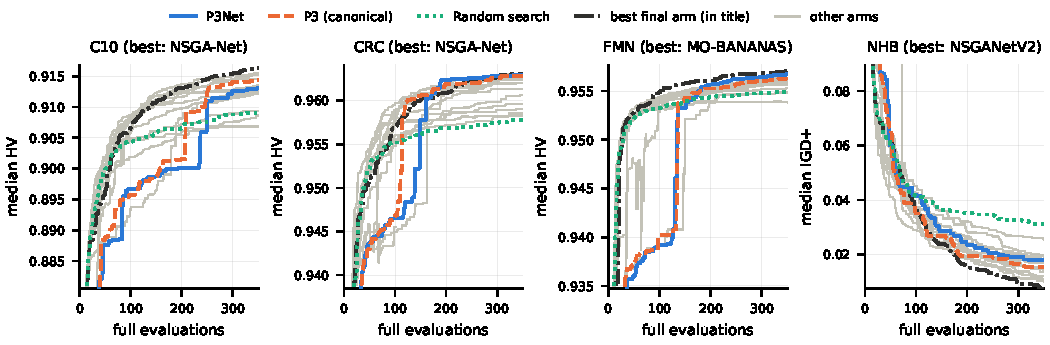
\includegraphics[width=\textwidth]{figures/anytime__primary__budget350.pdf}
    \caption{Anytime quality (pre-registration \S5.1), primary spaces, $b = 350$: median over 30 seeds of the primary metric after each full evaluation (HV higher is better, IGD+ lower is better; y-axis cut to the range after 20 evaluations). Grey: all other main-track arms; dash-dot: the arm with the best median final value in the space. Multi-fidelity arms are on a cost axis and are in the released \texttt{anytime.csv}.}
    \Description{Four line charts, one per primary search space, of median quality against the number of full evaluations up to 350, highlighting P3Net, canonical P3, random search and the best arm.}
    \label{fig:v005-s-anytime}
\end{figure*}



\end{document}
